% Appendix A

\chapter{Figures} % Main appendix title

\label{AppendixA} % For referencing this appendix elsewhere, use \ref{AppendixA}

% outline
%----------------------------------------------------------------------------
% 
%

\section{Best Result for Full Dataset}


\begin{figure}[htbp]
    \centering
    % First row: 4 figures
    \begin{subfigure}[b]{0.23\textwidth}
        \centering
        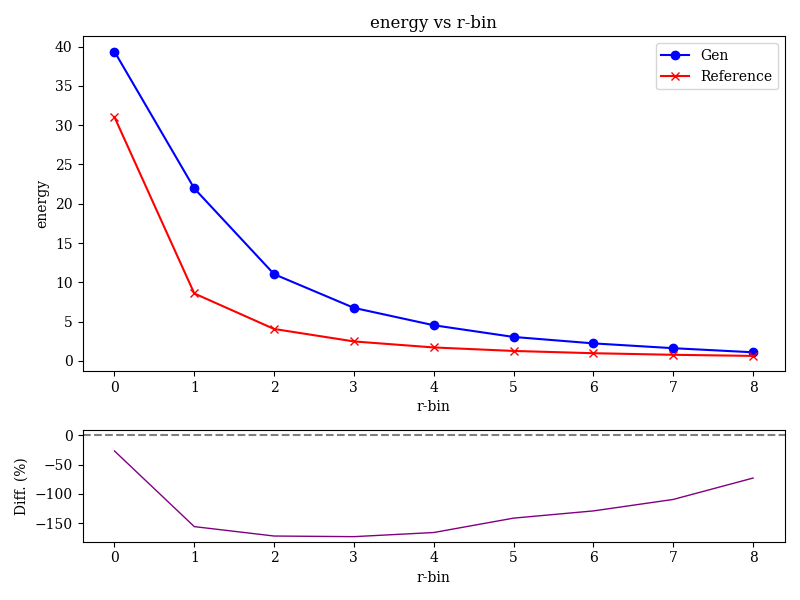
\includegraphics[width=\textwidth]{Figures/a1_2.png}
        \caption{Energy vs Radius}
        \label{fig:a1-2}
    \end{subfigure}
    \hfill
    \begin{subfigure}[b]{0.23\textwidth}
        \centering
        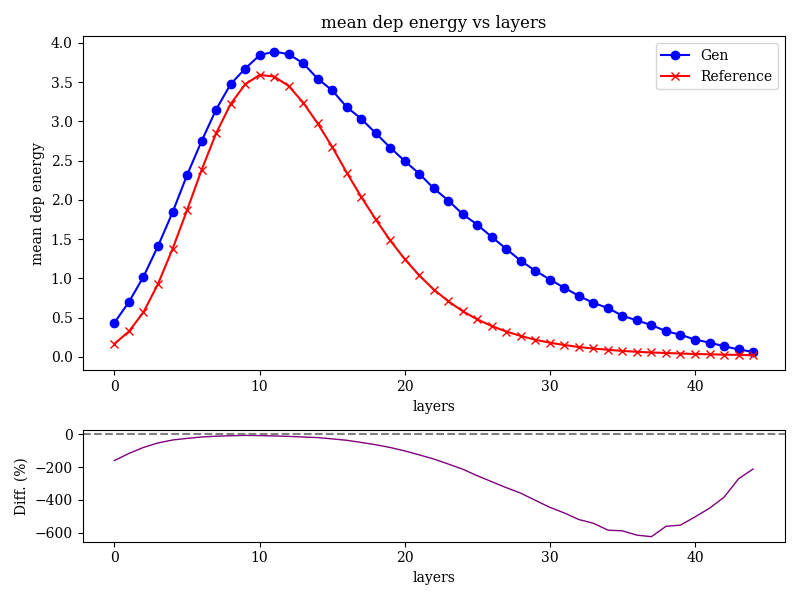
\includegraphics[width=\textwidth]{Figures/a1_3.png}
        \caption{Energy vs Z}
        \label{fig:a1-3}
    \end{subfigure}
    \hfill
    \begin{subfigure}[b]{0.23\textwidth}
        \centering
        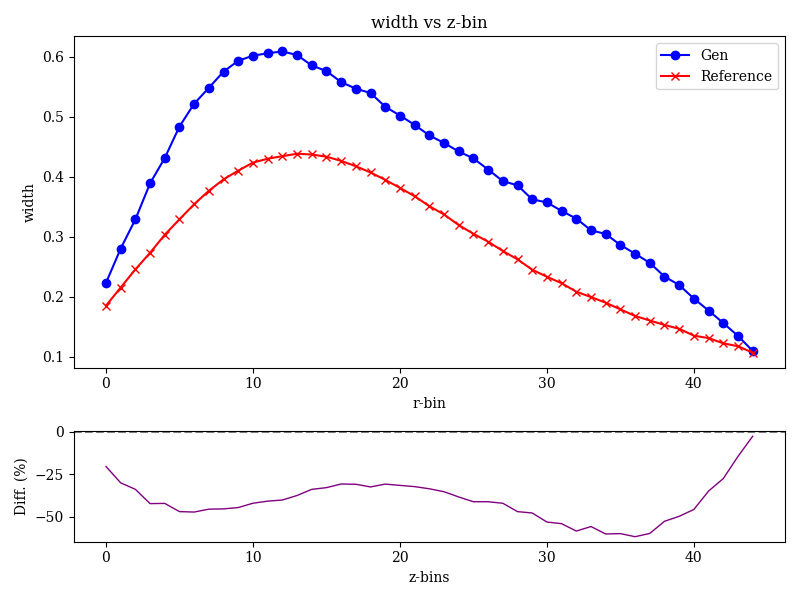
\includegraphics[width=\textwidth]{Figures/a1_4.png}
        \caption{R-width vs Layers}
        \label{fig:a1-4}
    \end{subfigure}
    \hfill
    \begin{subfigure}[b]{0.23\textwidth}  % Adjust width to fit 4 figures
        \centering
        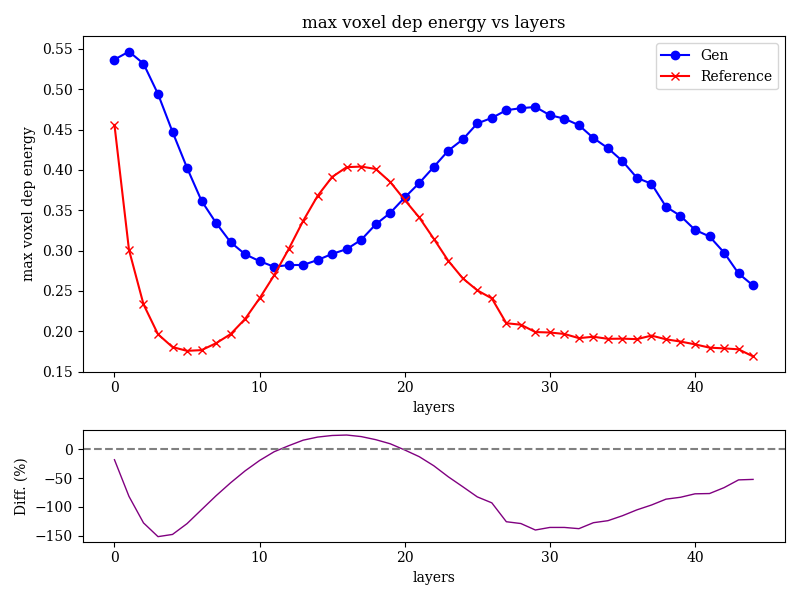
\includegraphics
        [width=\textwidth]{Figures/a1_5.png}
        \caption{Max Voxel Deposit vs Layers}
        
        \label{fig:a1-1}
    \end{subfigure}
    
    \vspace{0.6cm} % Space between rows

    % Second row: 3 figures
    \begin{subfigure}[b]{0.3\textwidth}  % Adjust width to fit 3 figures
        \centering
        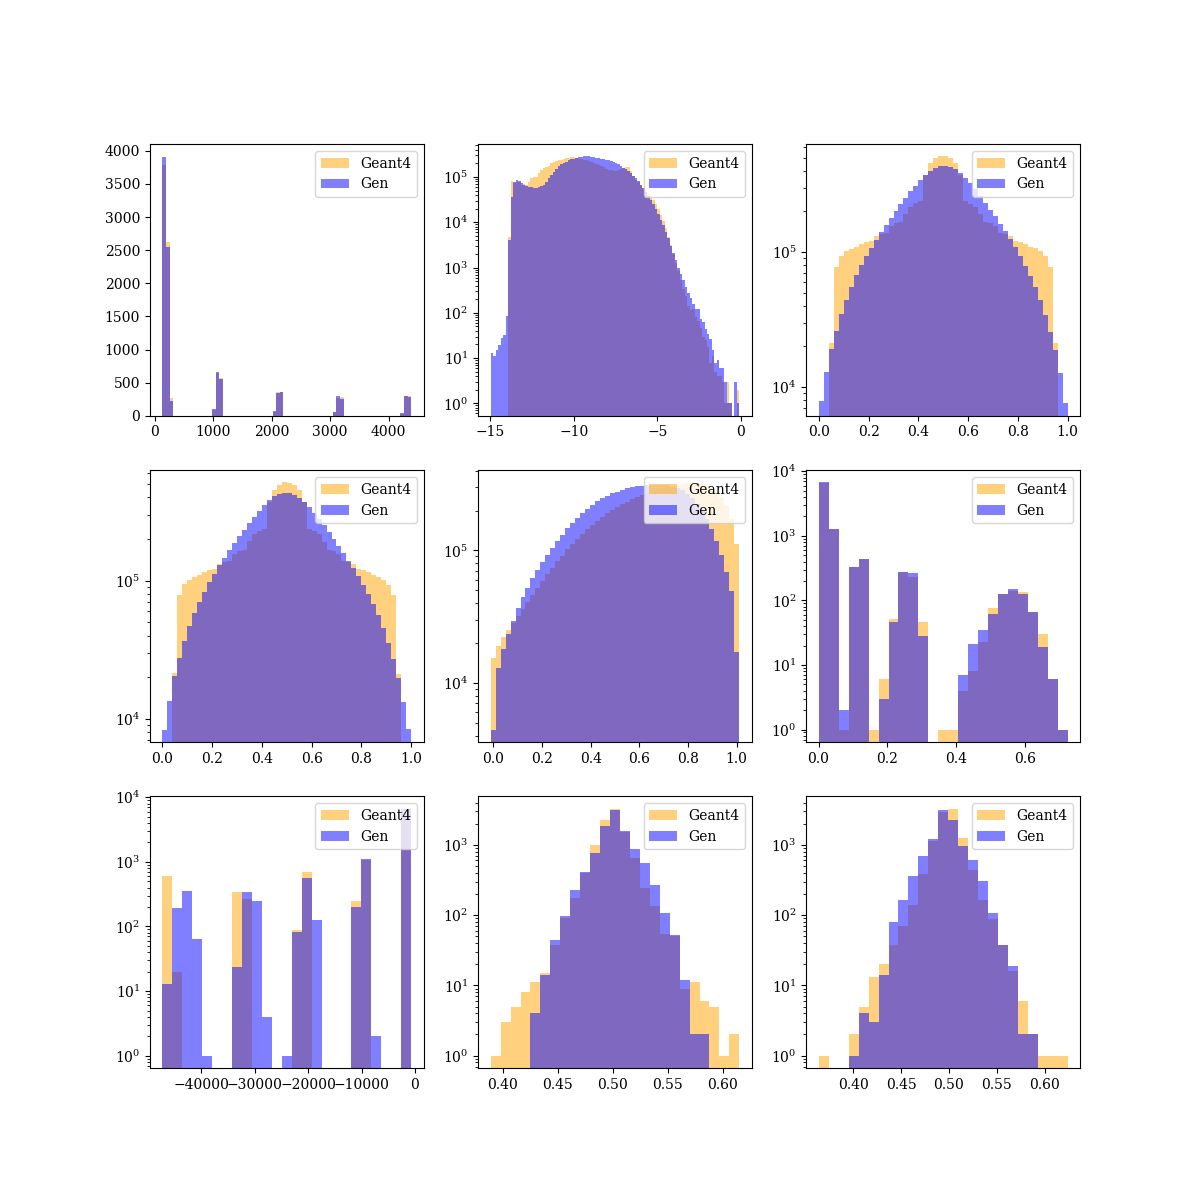
\includegraphics
        [width=\textwidth]{Figures/a1-1.png}
        \caption{1D Histogram}
        \label{fig:a1-5}
    \end{subfigure}
    \hfill
    \begin{subfigure}[b]{0.3\textwidth}
        \centering
        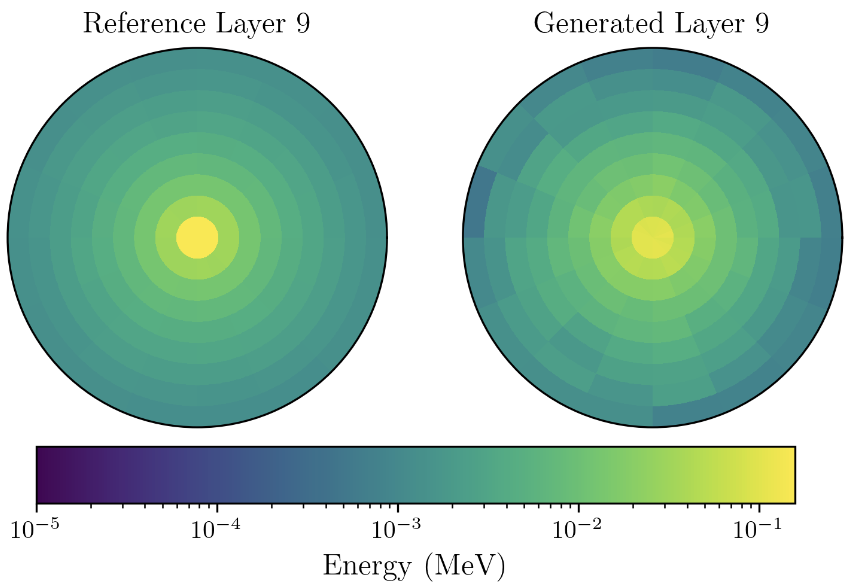
\includegraphics[width=\textwidth]{Figures/comparison.png}
        \caption{Energy voxel comparison}
        \label{fig:a1_5}
    \end{subfigure}
    \hfill
    \begin{subfigure}[b]{0.3\textwidth}
        \centering
        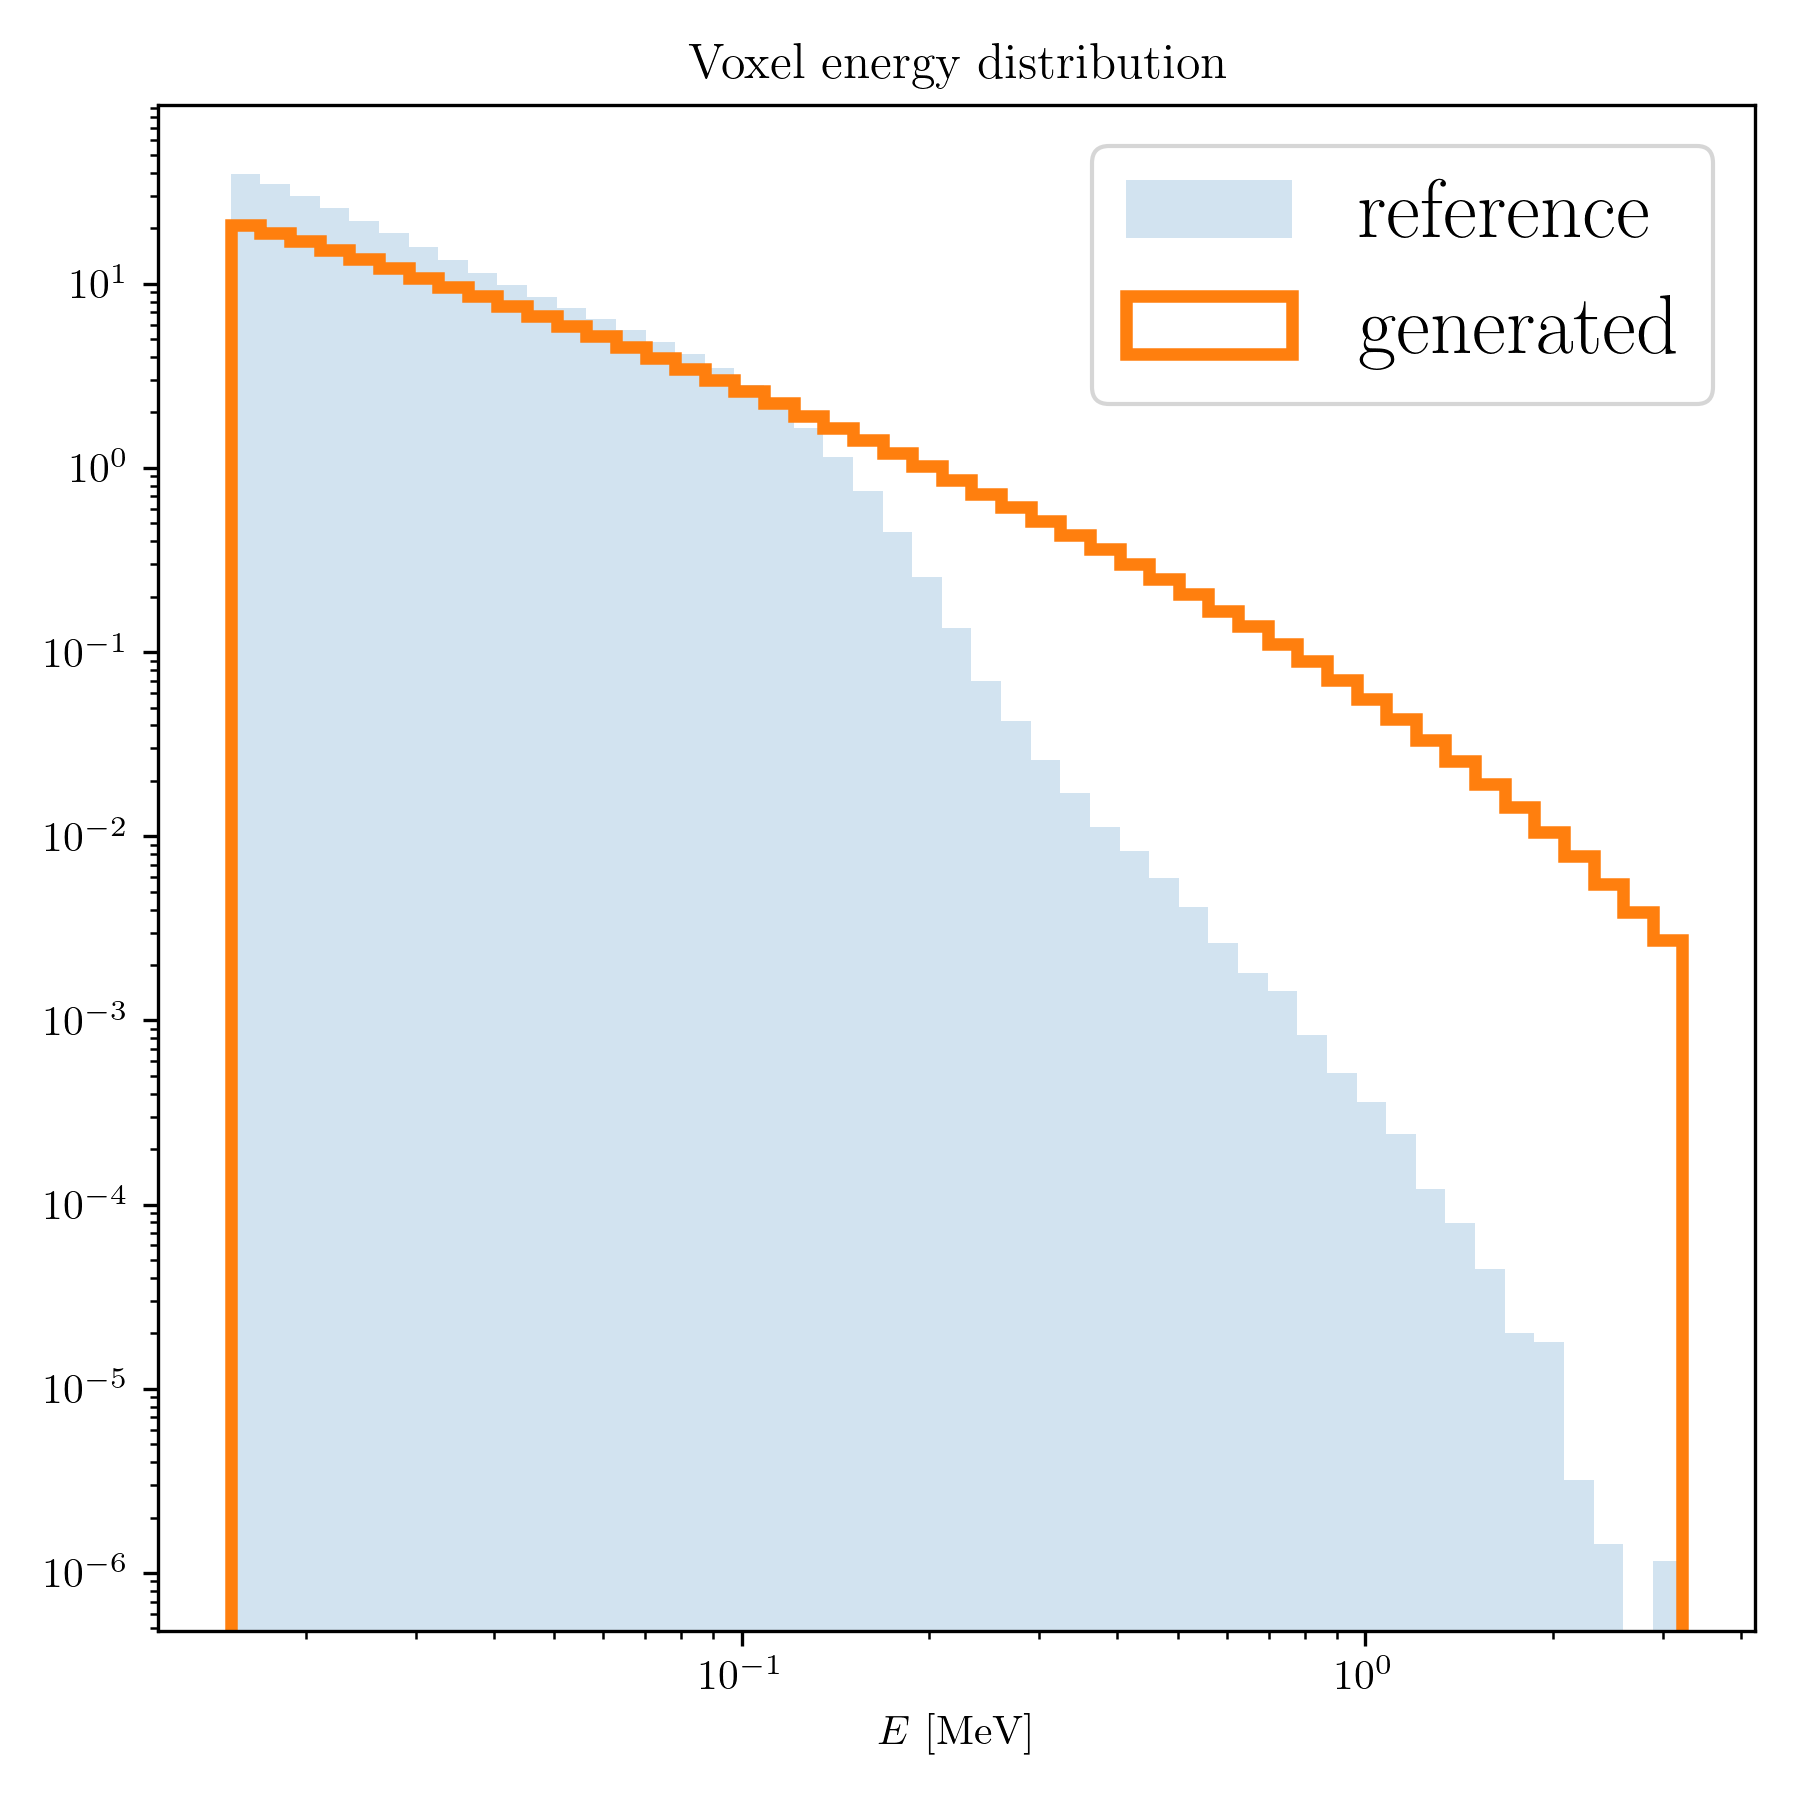
\includegraphics[width=\textwidth]{Figures/a1_7.png}
        \caption{Energy Deposit}
        \label{fig:a1_7}
    \end{subfigure}
\end{figure}

\newpage
\section{Best Result for Single Bucket Data}


\begin{figure}[htbp]
    \centering
    % First row: 4 figures
    \begin{subfigure}[b]{0.23\textwidth}
        \centering
        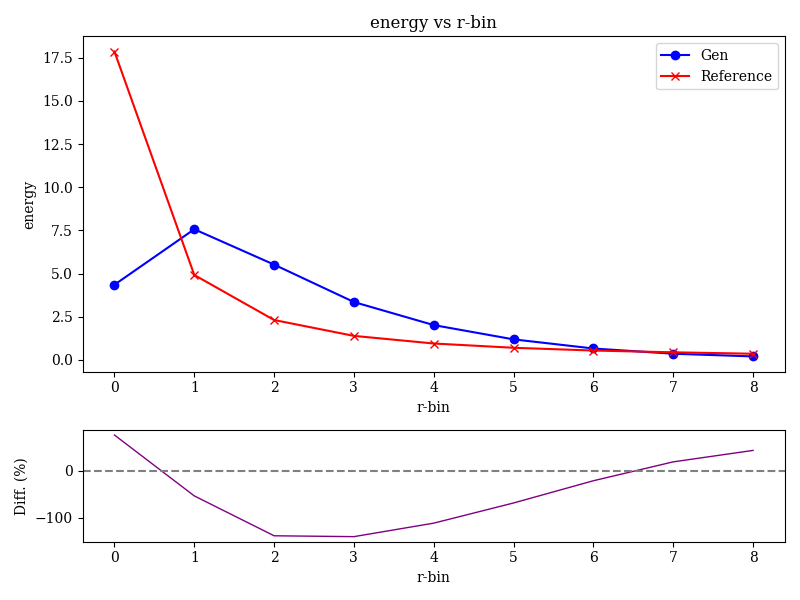
\includegraphics[width=\textwidth]{Figures/2_2.png}
        \caption{Energy vs Radius}
        \label{fig:a2_2}
    \end{subfigure}
    \hfill
    \begin{subfigure}[b]{0.23\textwidth}
        \centering
        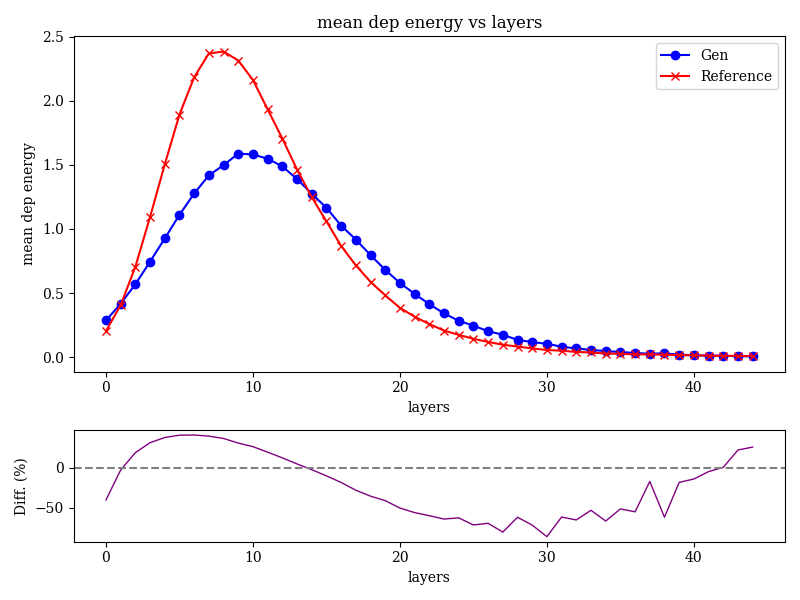
\includegraphics[width=\textwidth]{Figures/2_3.png}
        \caption{Energy vs Z}
        \label{fig:a2_3}
    \end{subfigure}
    \hfill
    \begin{subfigure}[b]{0.23\textwidth}
        \centering
        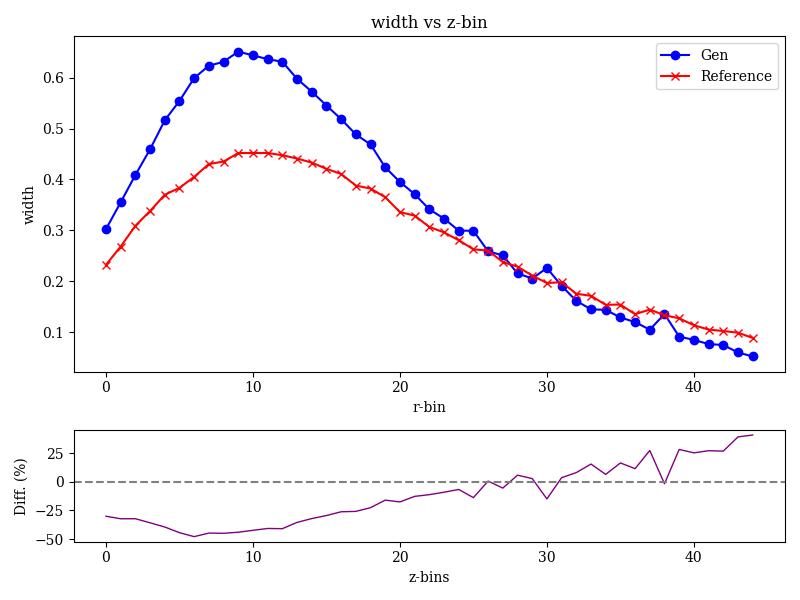
\includegraphics[width=\textwidth]{Figures/2_4.png}
        \caption{R-width vs layers}
        \label{fig:a2_4}
    \end{subfigure}
    \hfill
    \begin{subfigure}[b]{0.23\textwidth}  % Adjust width to fit 4 figures
        \centering
        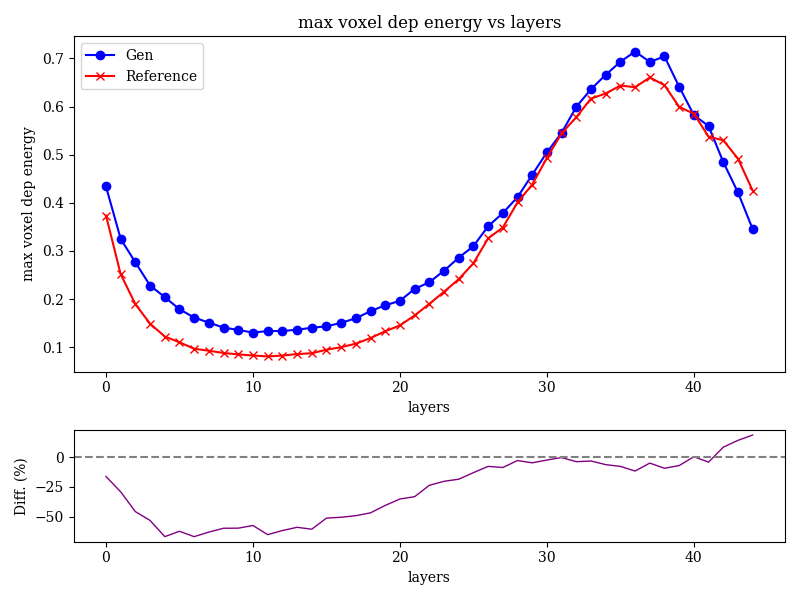
\includegraphics
        [width=\textwidth]{Figures/2_5.png}
        \caption{Max Voxel Deposit vs Layers}
        \label{fig:a2_1}
    \end{subfigure}

    \vspace{0.6cm} % Space between rows

    % Second row: 3 figures
    \begin{subfigure}[b]{0.3\textwidth}  % Adjust width to fit 3 figures
        \centering
        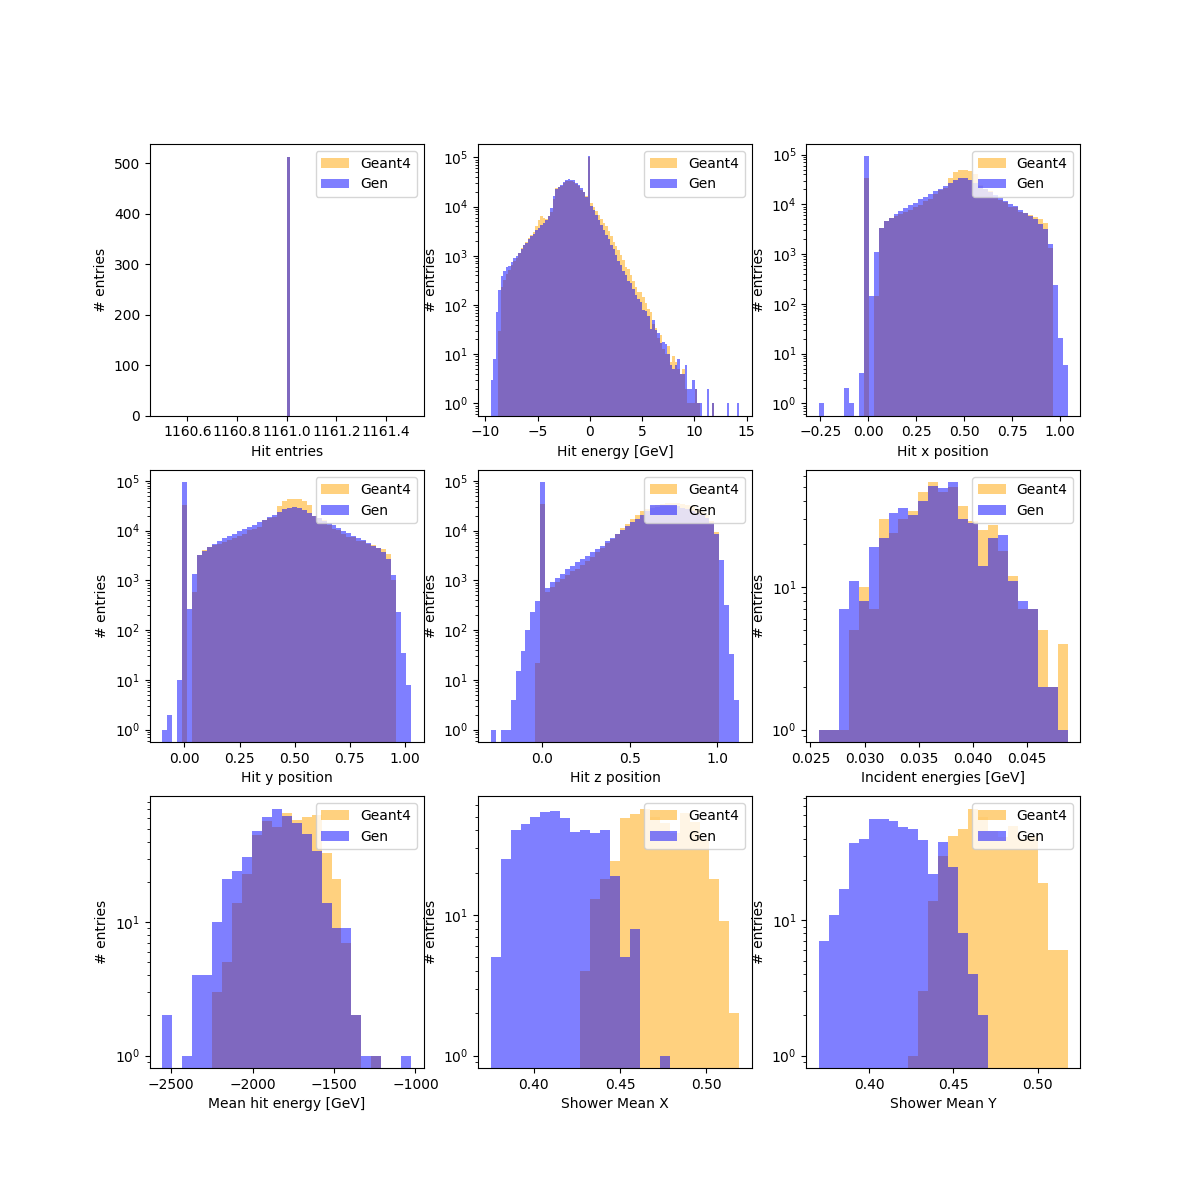
\includegraphics
        [width=\textwidth]{Figures/a2_1.png}
        \caption{1D Histogram}
        \label{fig:a2_5}
    \end{subfigure}
    \hfill
    \begin{subfigure}[b]{0.3\textwidth}
        \centering
        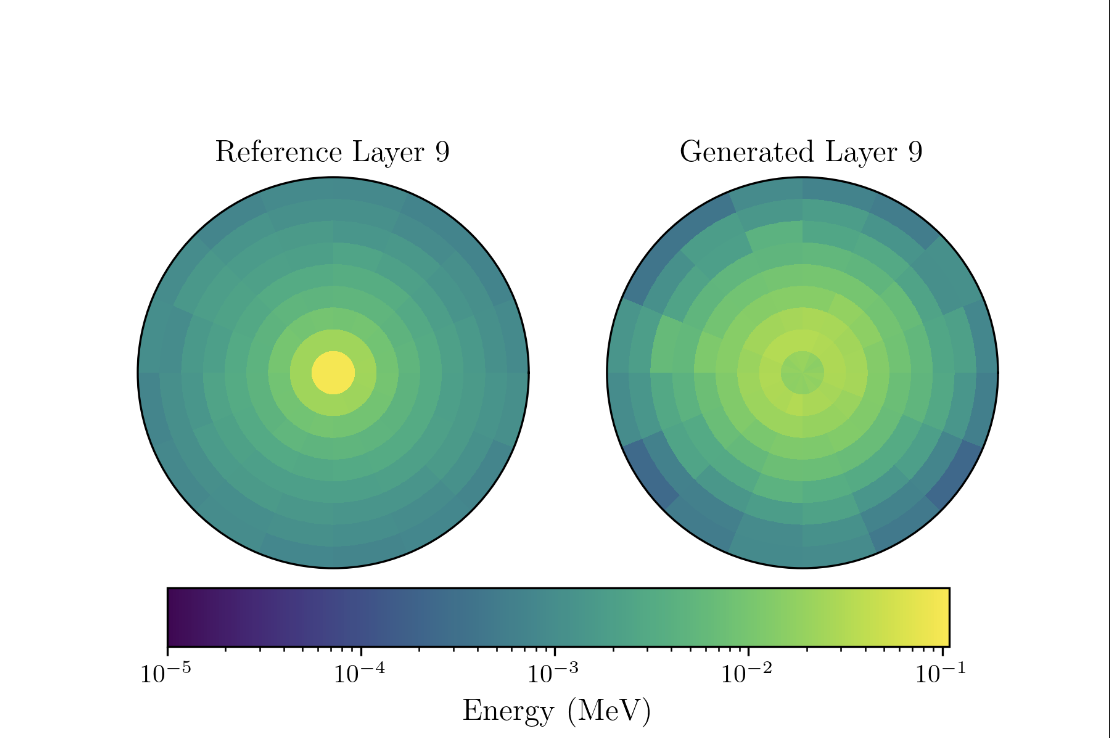
\includegraphics[width=\textwidth]{Figures/a2_5.png}
        \caption{Energy voxel comparison}
        \label{fig:a2_6}
    \end{subfigure}
    \hfill
    \begin{subfigure}[b]{0.3\textwidth}
        \centering
        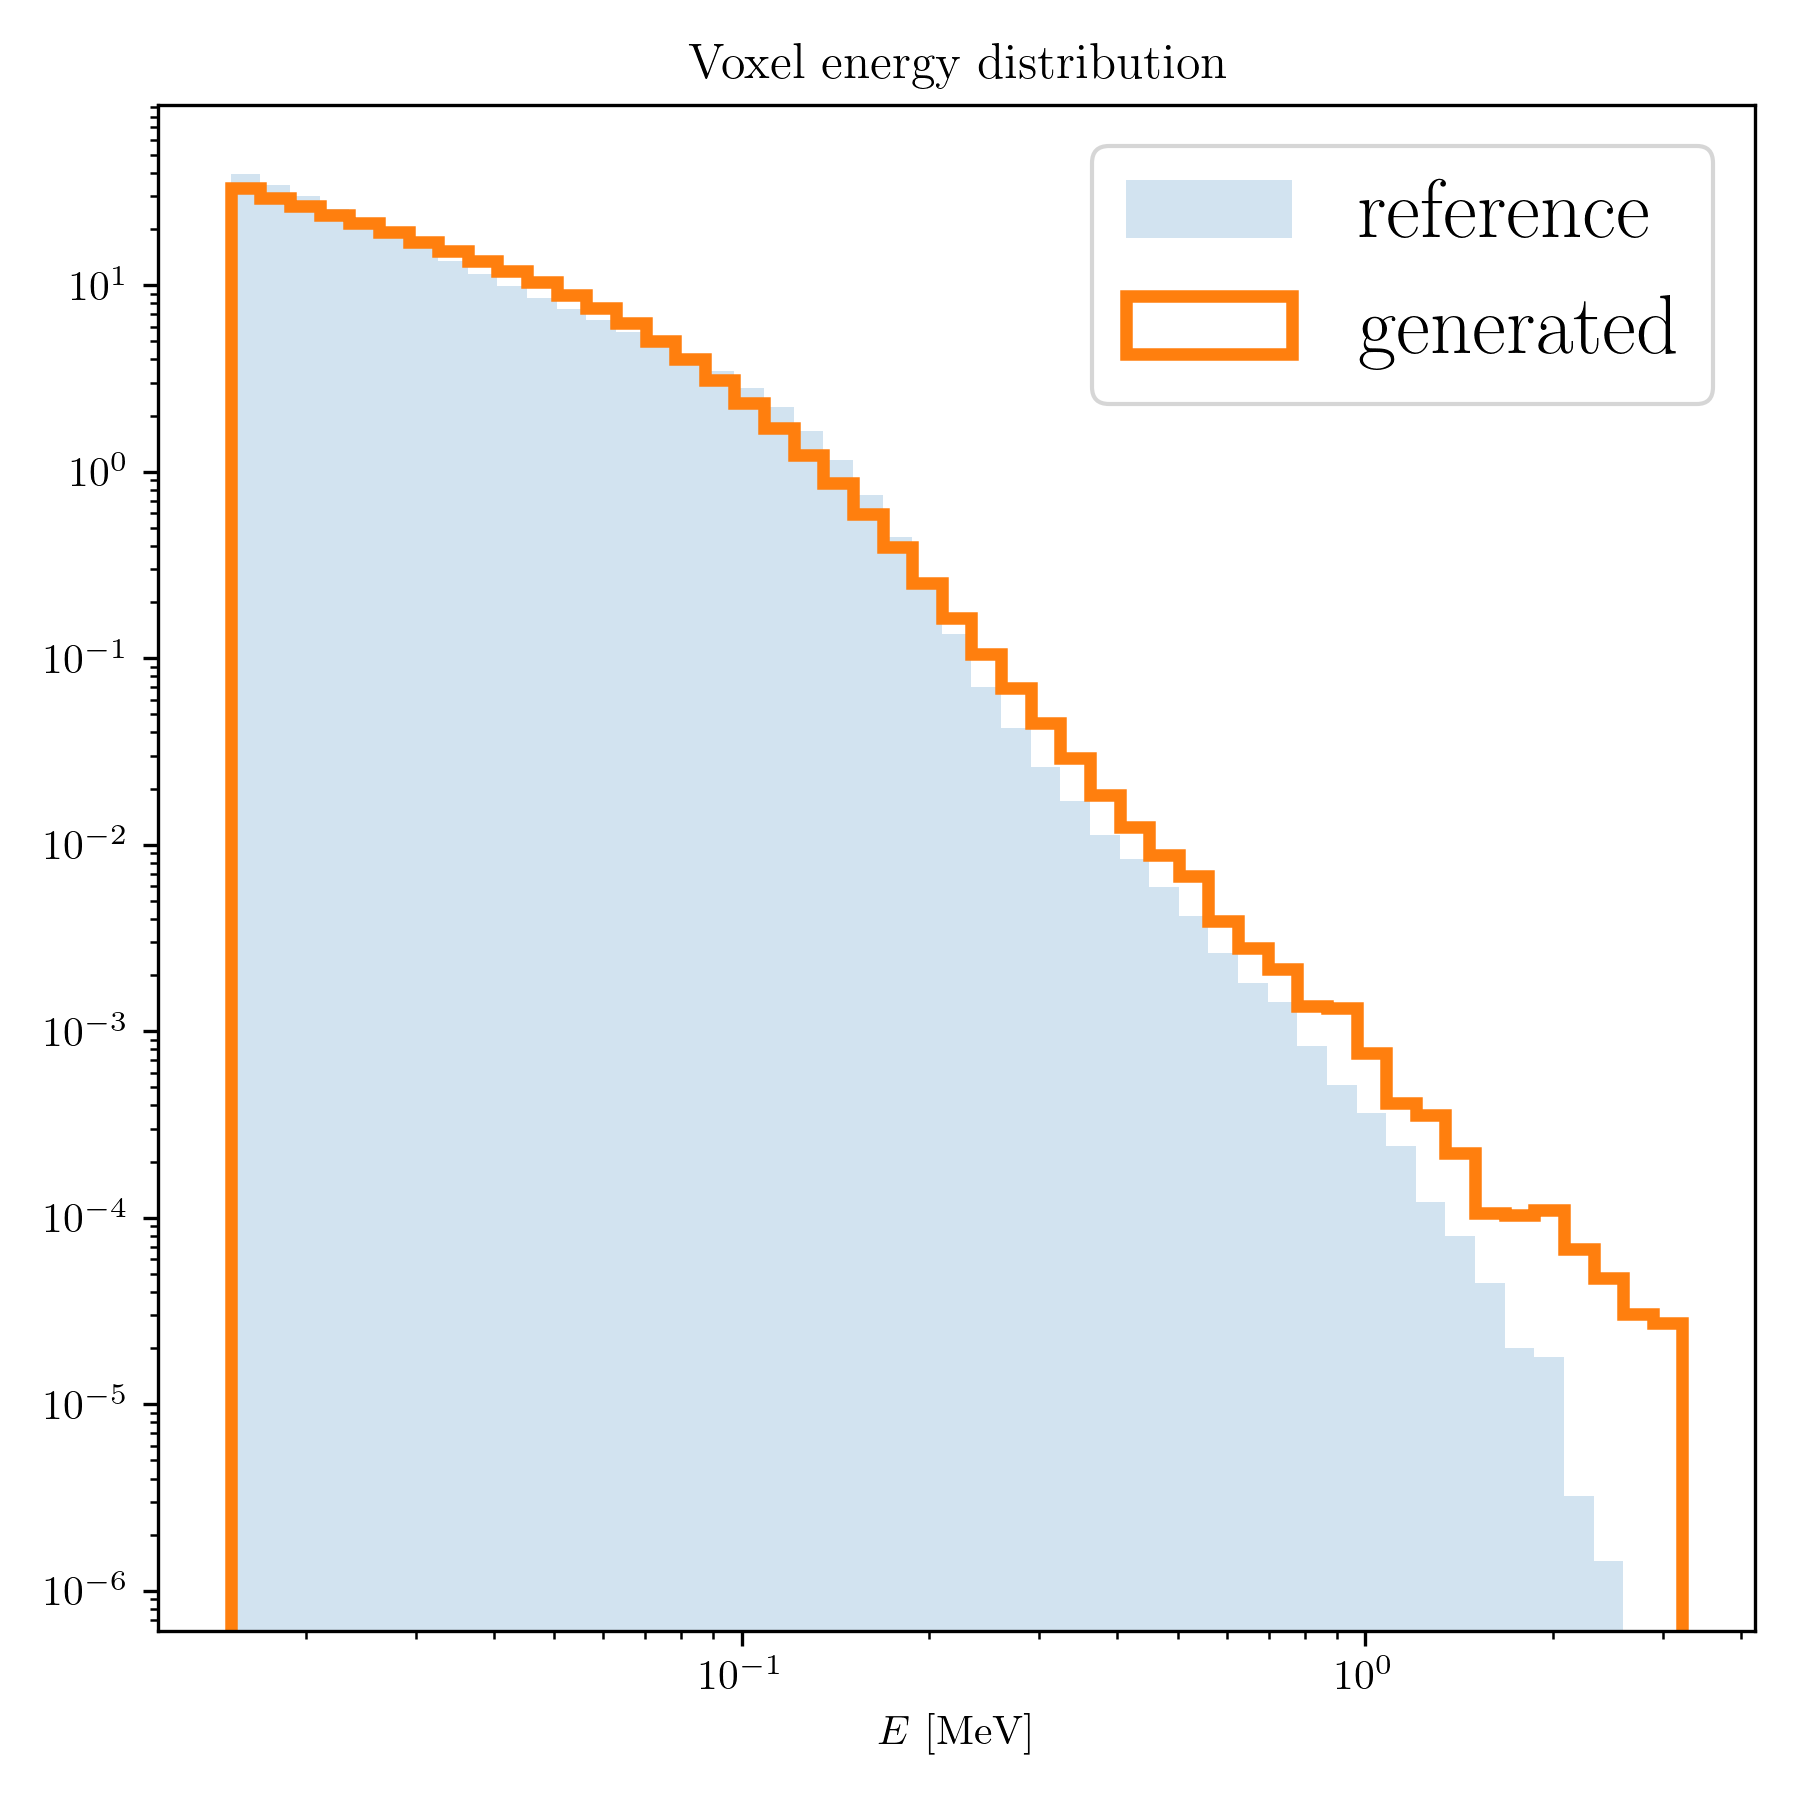
\includegraphics[width=\textwidth]{Figures/a2_6.png}
        \caption{Energy Deposit}
        \label{fig:a2_7}
    \end{subfigure}
\end{figure}
% \section{Result for without using incident energy}
% 7 pictures in total
\newpage
\section{Result for using different Preprocessor}


\begin{figure}[htbp]
    \centering
    % First row: 4 figures
    \begin{subfigure}[b]{0.3\textwidth}
        \centering
        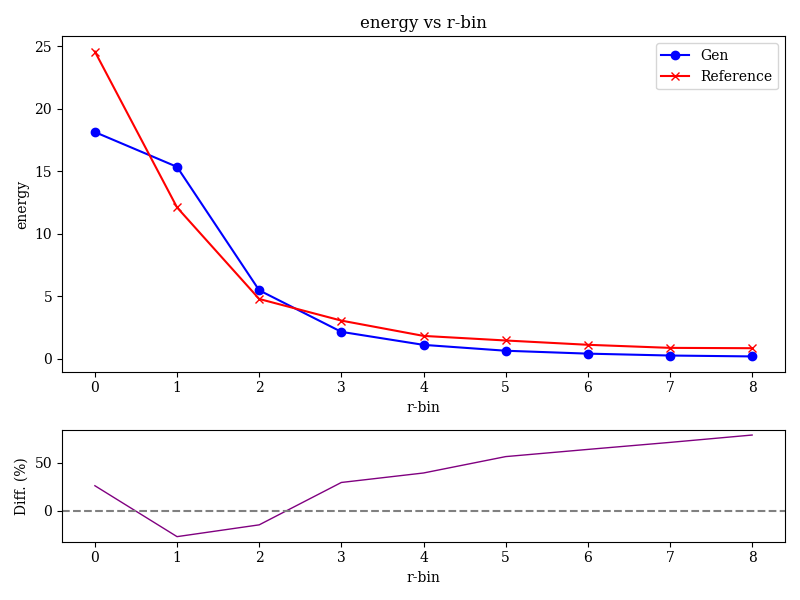
\includegraphics[width=\textwidth]{Figures/robust2.png}
        \caption{Energy vs Radius}
        \label{fig:robust2}
    \end{subfigure}
    \hfill
    \begin{subfigure}[b]{0.3\textwidth}
        \centering
        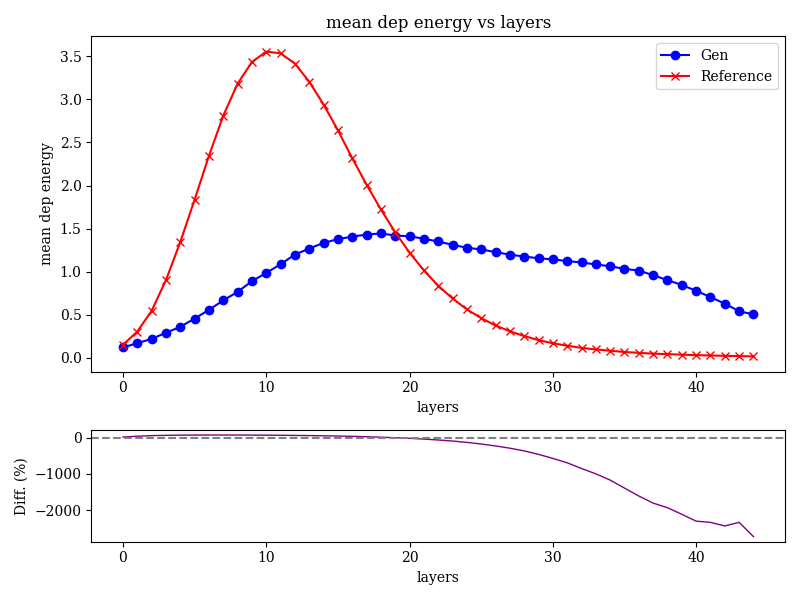
\includegraphics[width=\textwidth]{Figures/robust3.png}
        \caption{Energy vs Z}
        \label{fig:robust3}
    \end{subfigure}
    \hfill
    \begin{subfigure}[b]{0.3\textwidth}
        \centering
        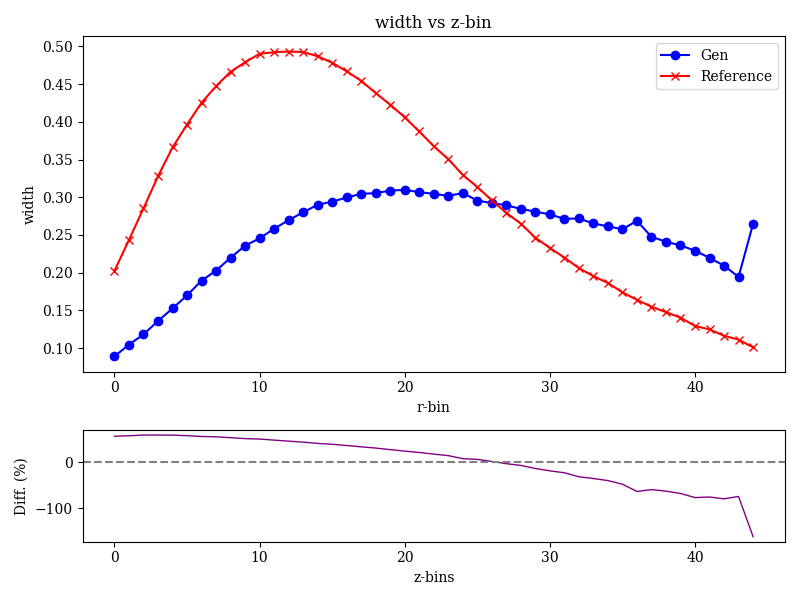
\includegraphics[width=\textwidth]{Figures/robust4.png}
        \caption{R-width vs layers}
        \label{fig:robust4}
    \end{subfigure}
    

    \vspace{0.35cm} % Space between rows

    % Second row: 3 figures
    
    \begin{subfigure}[b]{0.3\textwidth}  % Adjust width to fit 4 figures
        \centering
        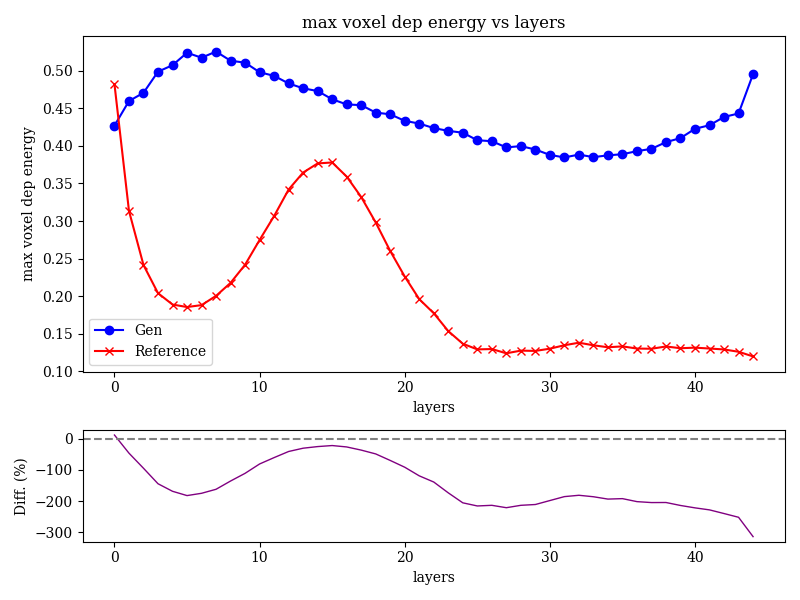
\includegraphics
        [width=\textwidth]{Figures/robust5.png}
        \caption{Max Voxel Deposit vs Layers}
        \label{fig:robust5}
    \end{subfigure}
    \hfill
    \begin{subfigure}[b]{0.3\textwidth}  % Adjust width to fit 3 figures
        \centering
        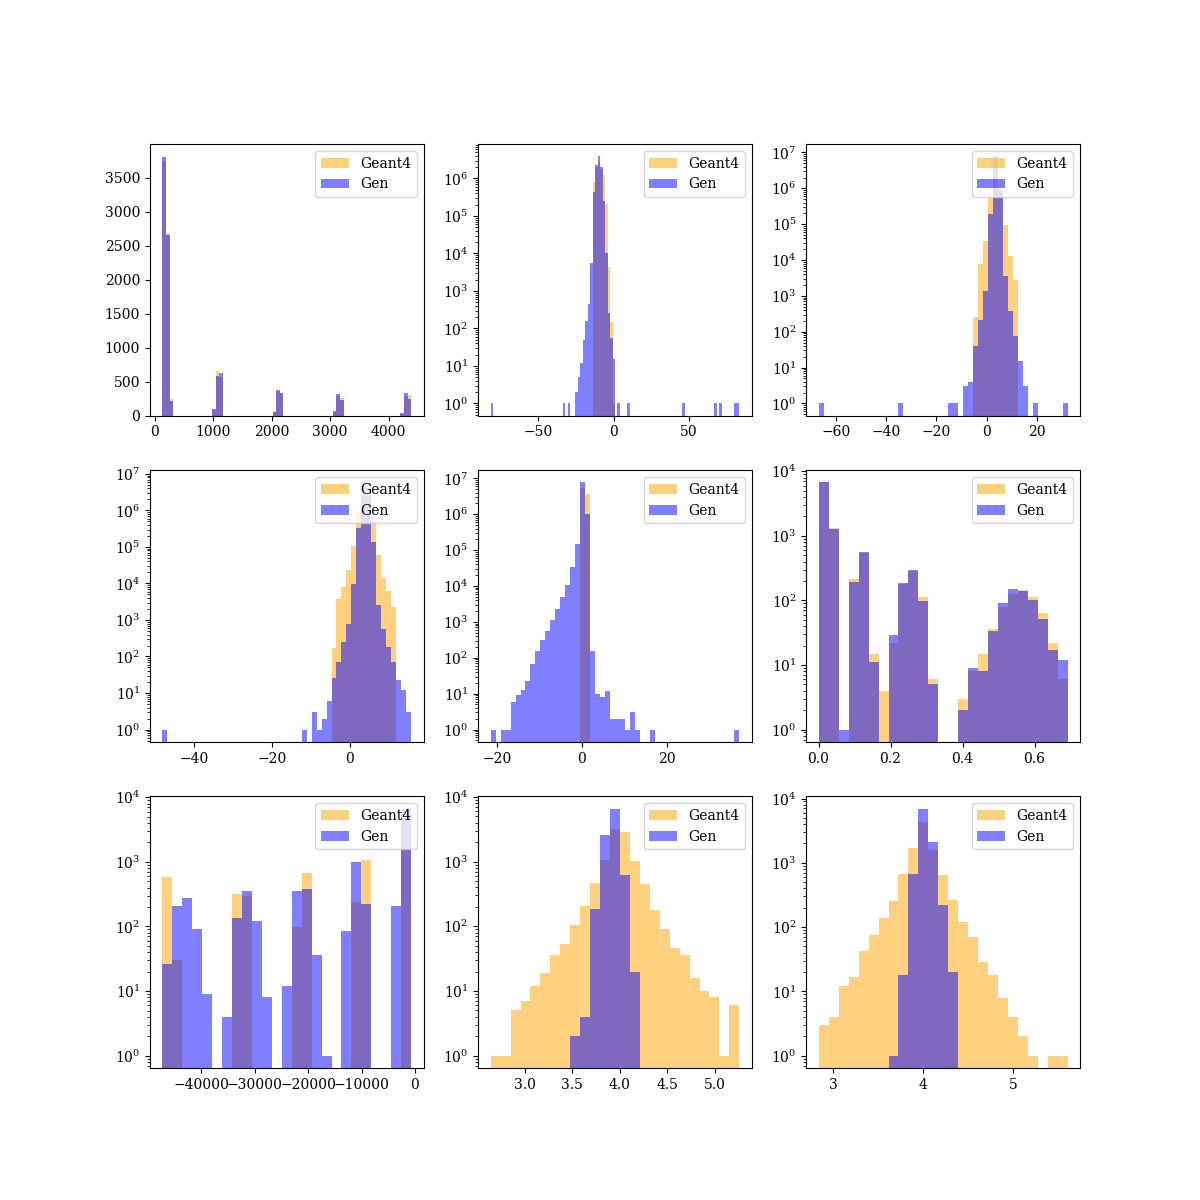
\includegraphics
        [width=\textwidth]{Figures/robust1.png}
        \caption{1D Histogram}
        \label{fig:robust1}
    \end{subfigure}
    \hfill
    \begin{subfigure}[b]{0.3\textwidth}
        \centering
        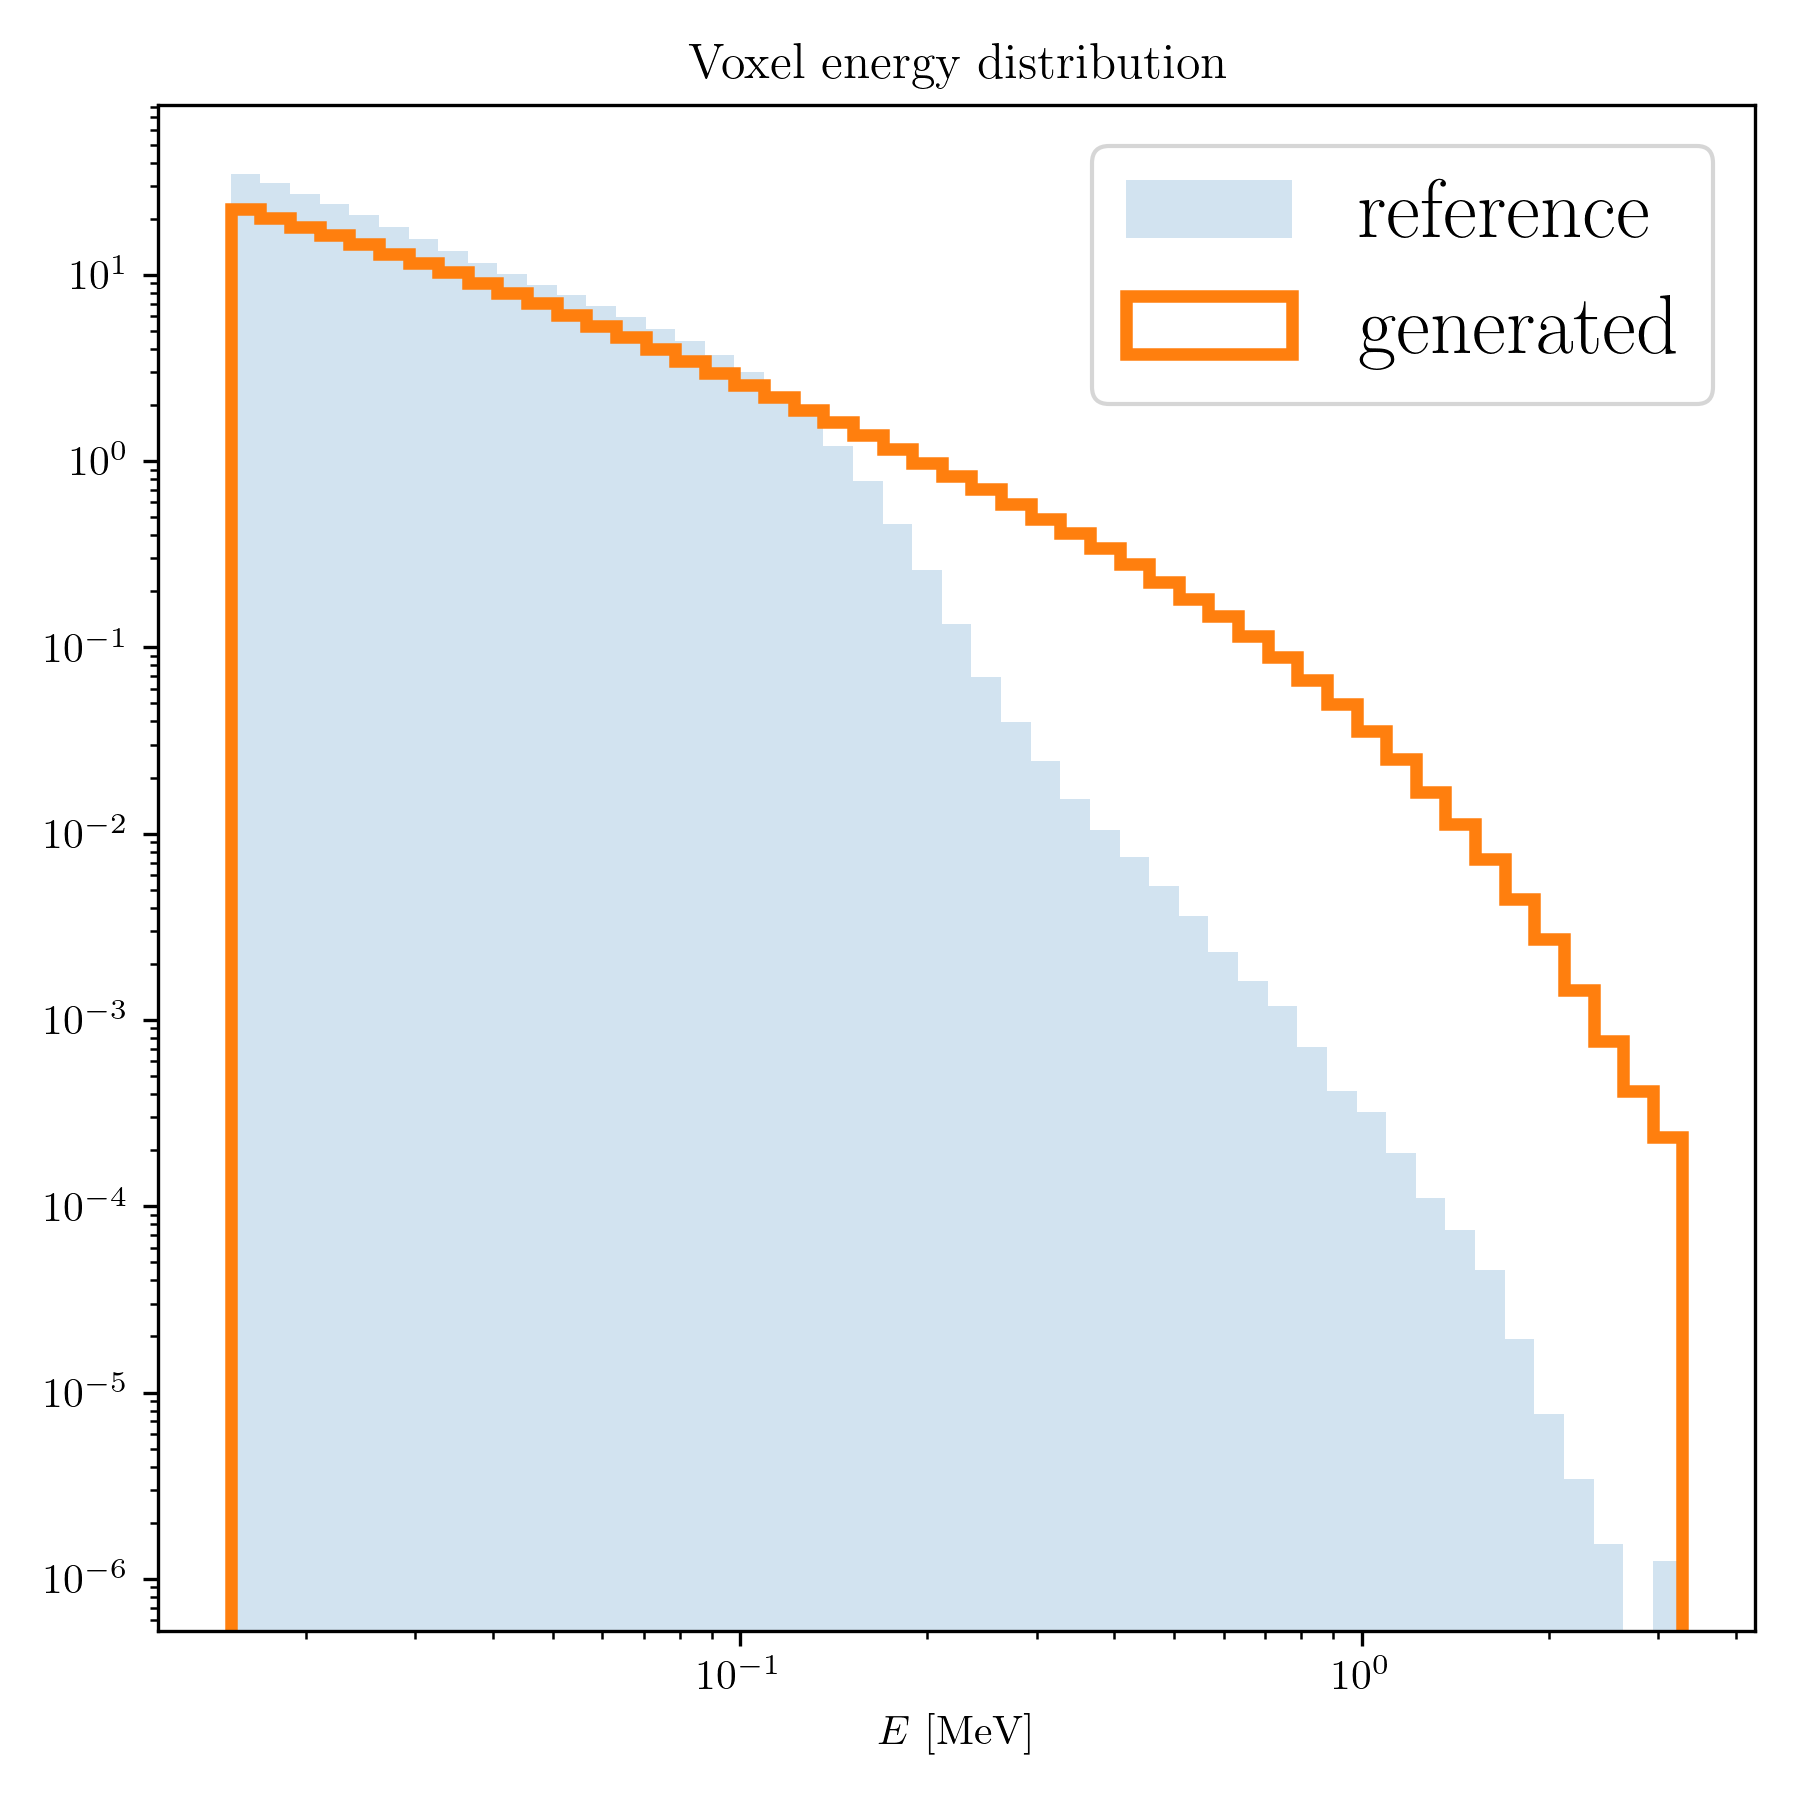
\includegraphics[width=\textwidth]{Figures/robust6.png}
        \caption{Energy Deposit}
        \label{fig:robust6}
    \end{subfigure}
    \caption{Result for using robust preprocessor}
\end{figure}

\begin{figure}
    \centering
    % First row: 4 figures
    \begin{subfigure}[b]{0.3\textwidth}
        \centering
        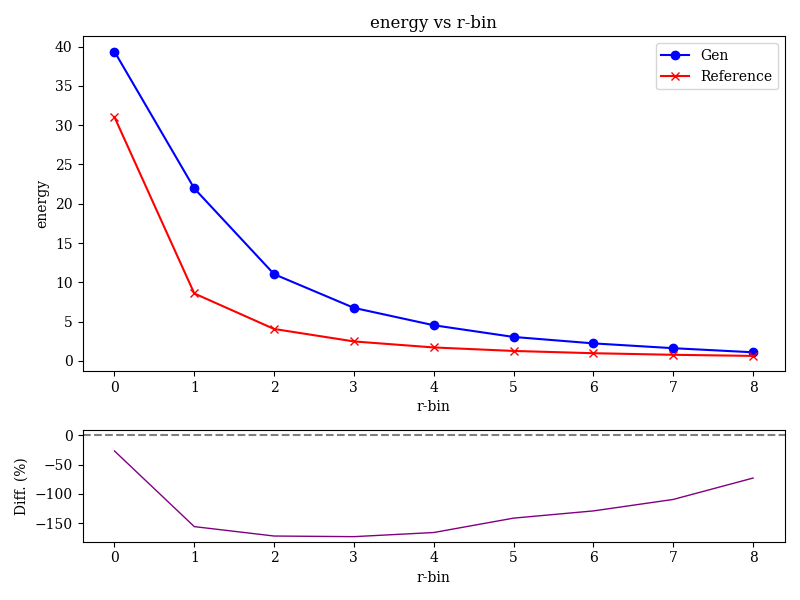
\includegraphics[width=\textwidth]{Figures/quantile2.png}
        \caption{Energy vs Radius}
        \label{fig:quantile2}
    \end{subfigure}
    \hfill
    \begin{subfigure}[b]{0.3\textwidth}
        \centering
        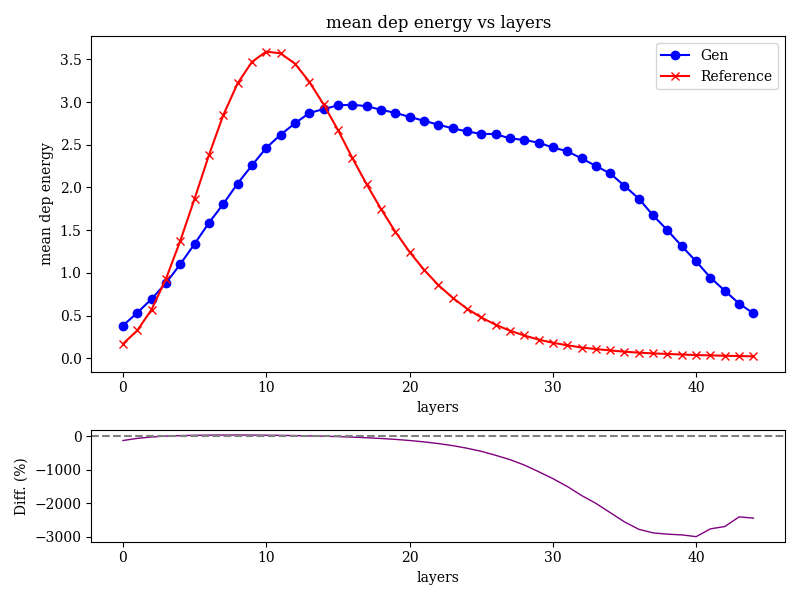
\includegraphics[width=\textwidth]{Figures/quantile3.png}
        \caption{Energy vs Z}
        \label{fig:quantile3}
    \end{subfigure}
    \hfill
    \begin{subfigure}[b]{0.3\textwidth}
        \centering
        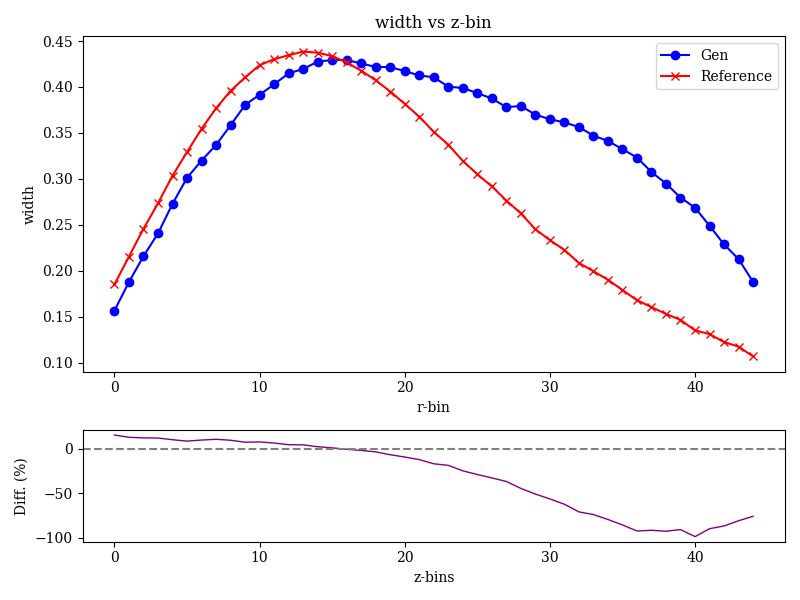
\includegraphics[width=\textwidth]{Figures/quantile4.png}
        \caption{R-width vs layers}
        \label{fig:quantile4}
    \end{subfigure}
    

    \vspace{0.35cm} % Space between rows

    % Second row: 3 figures
    
    \begin{subfigure}[b]{0.3\textwidth}  % Adjust width to fit 4 figures
        \centering
        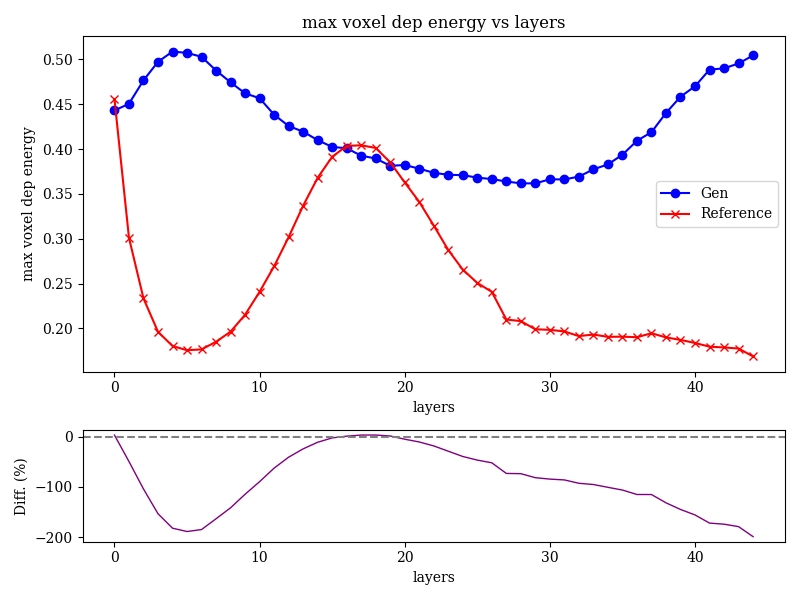
\includegraphics
        [width=\textwidth]{Figures/quantile5.png}
        \caption{Max Voxel Deposit vs Layers}
        \label{fig:quantile5}
    \end{subfigure}
    \hfill
    \begin{subfigure}[b]{0.3\textwidth}  % Adjust width to fit 3 figures
        \centering
        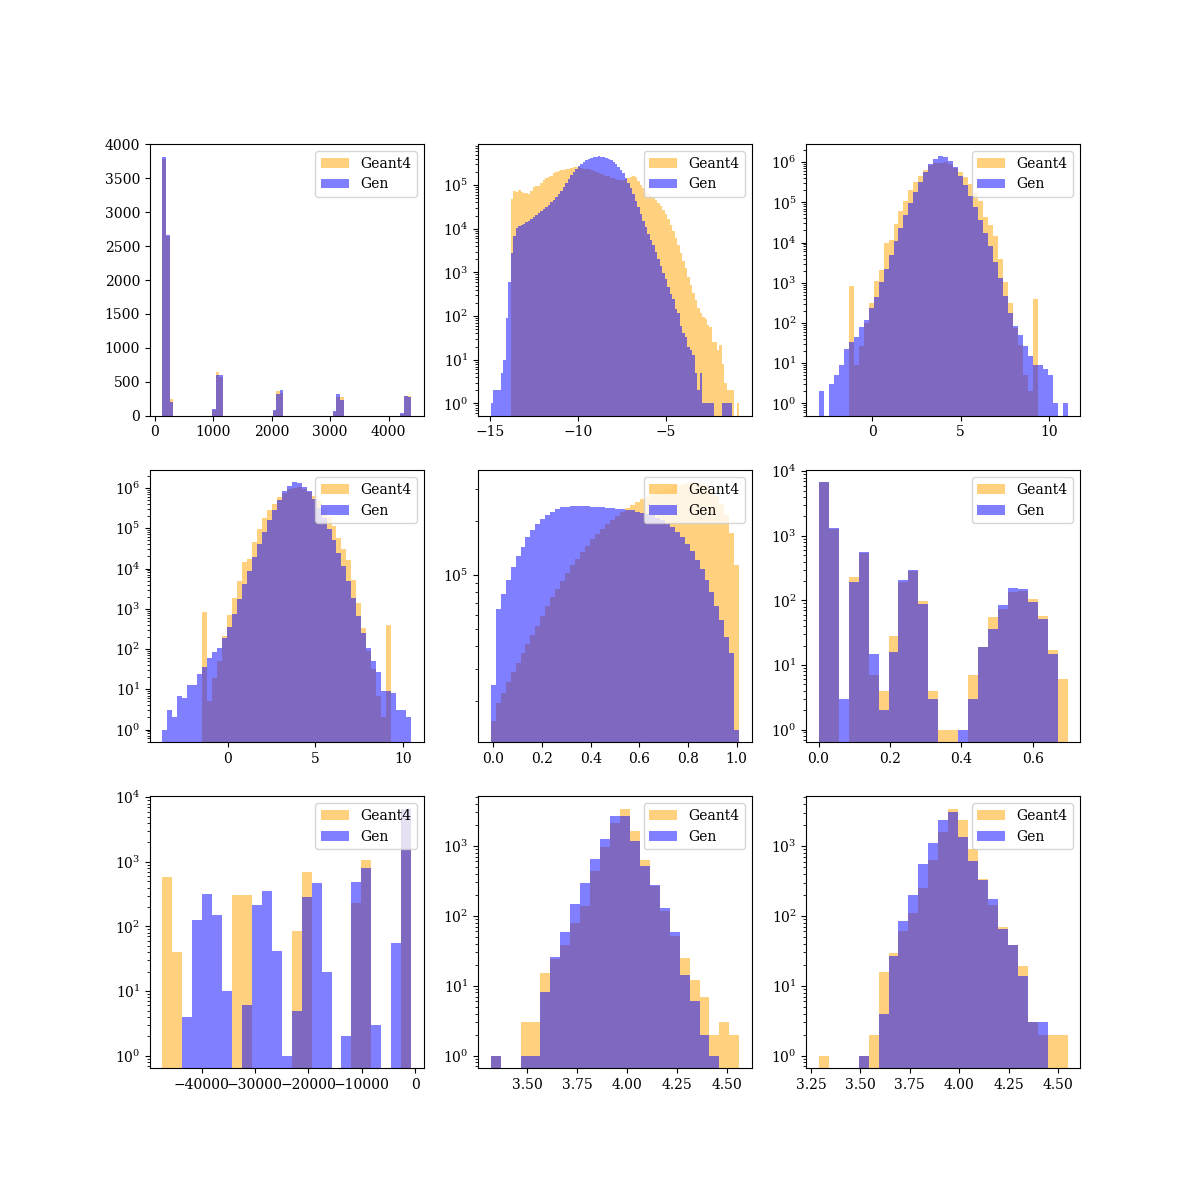
\includegraphics
        [width=\textwidth]{Figures/quantile1.png}
        \caption{1D Histogram}
        \label{fig:quantile1}
    \end{subfigure}
    \hfill
    \begin{subfigure}[b]{0.3\textwidth}
        \centering
        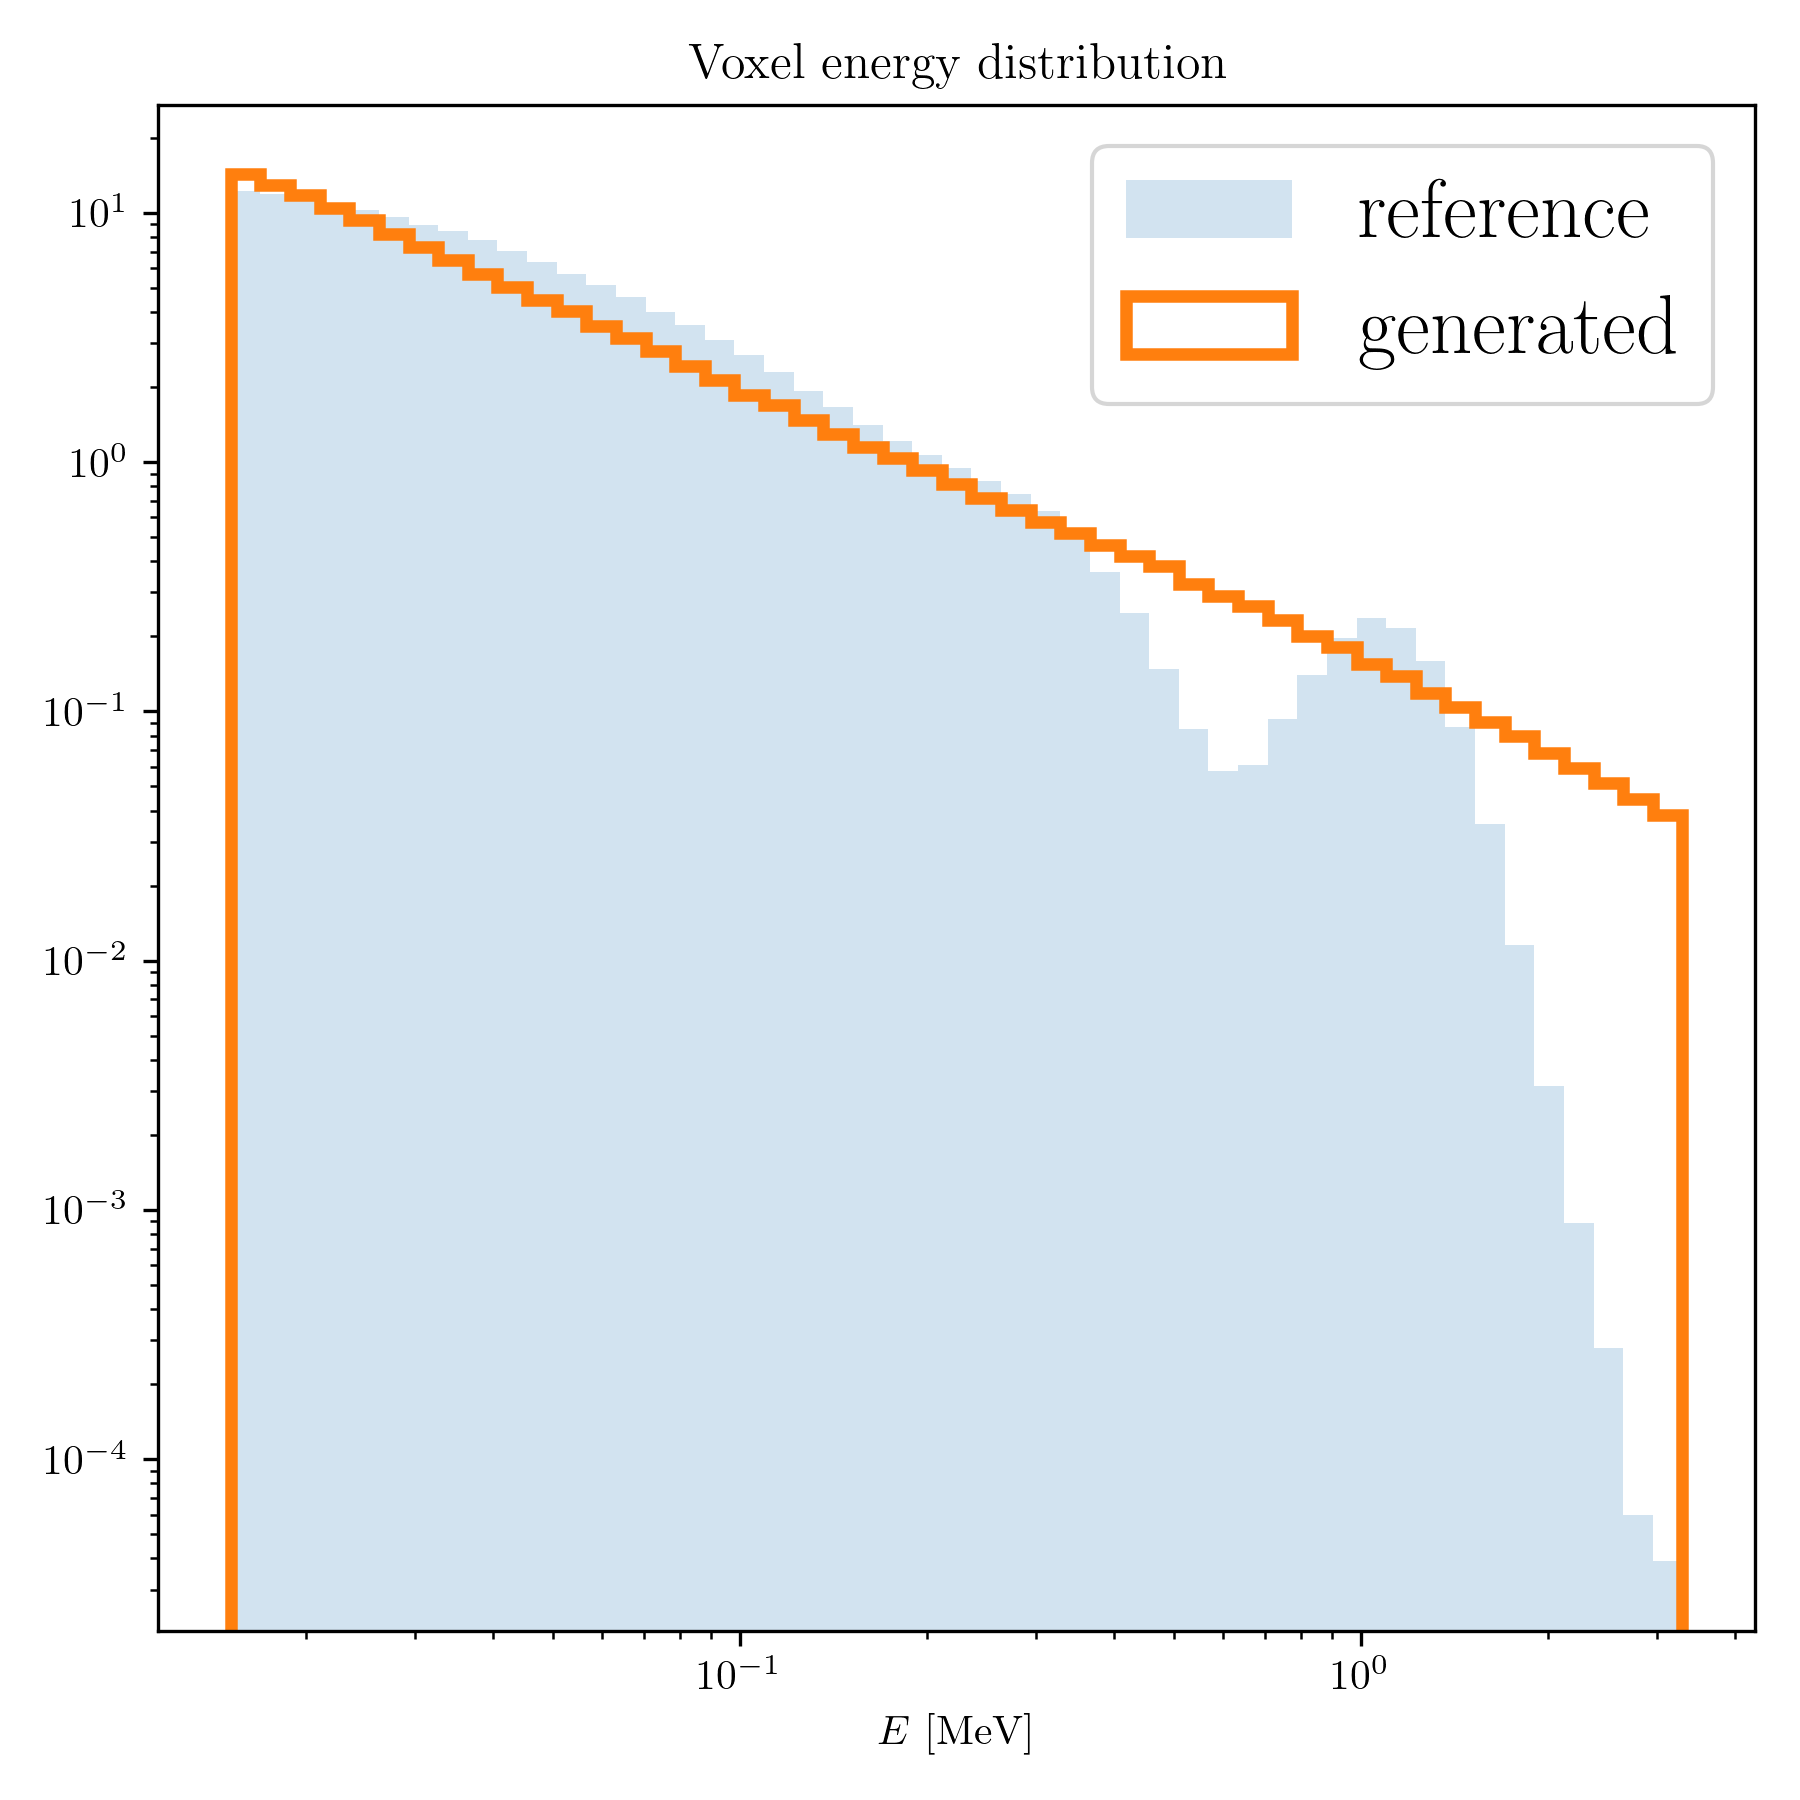
\includegraphics[width=\textwidth]{Figures/quantile6.png}
        \caption{Energy Deposit}
        \label{fig:quantile6}
    \end{subfigure}
    \caption{Result for using quantile preprocessor}
\end{figure}

\begin{figure}
    \centering
    % First row: 4 figures
    \begin{subfigure}[b]{0.3\textwidth}
        \centering
        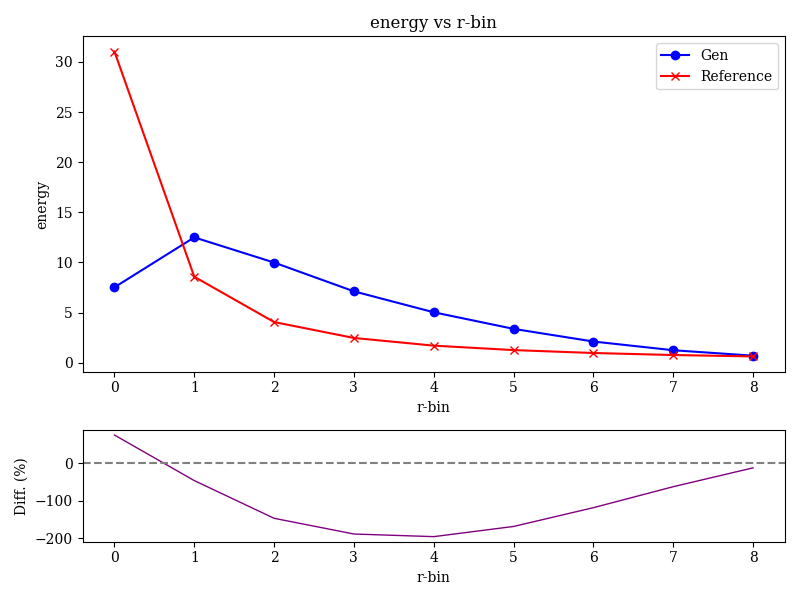
\includegraphics[width=\textwidth]{Figures/exponential2.png}
        \caption{Energy vs Radius}
        \label{fig:exp2}
    \end{subfigure}
    \hfill
    \begin{subfigure}[b]{0.3\textwidth}
        \centering
        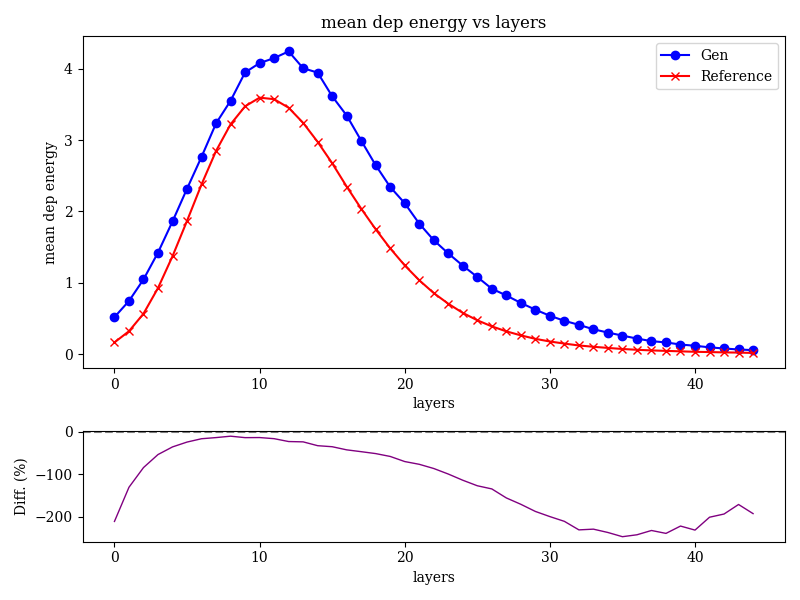
\includegraphics[width=\textwidth]{Figures/exponential3.png}
        \caption{Energy vs Z}
        \label{fig:exp3}
    \end{subfigure}
    \hfill
    \begin{subfigure}[b]{0.3\textwidth}
        \centering
        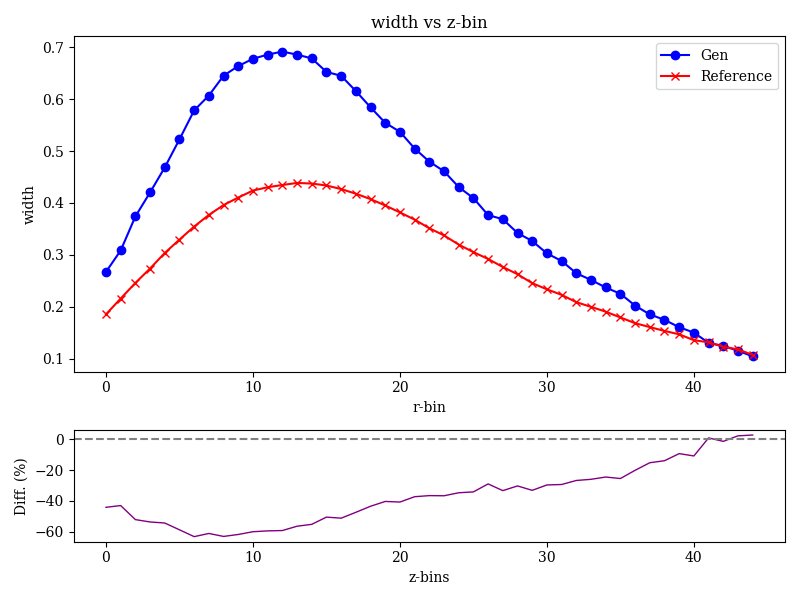
\includegraphics[width=\textwidth]{Figures/exponential4.png}
        \caption{R-width vs layers}
        \label{fig:exp4}
    \end{subfigure}
    

    \vspace{0.35cm} % Space between rows

    % Second row: 3 figures
    
    \begin{subfigure}[b]{0.3\textwidth}  % Adjust width to fit 4 figures
        \centering
        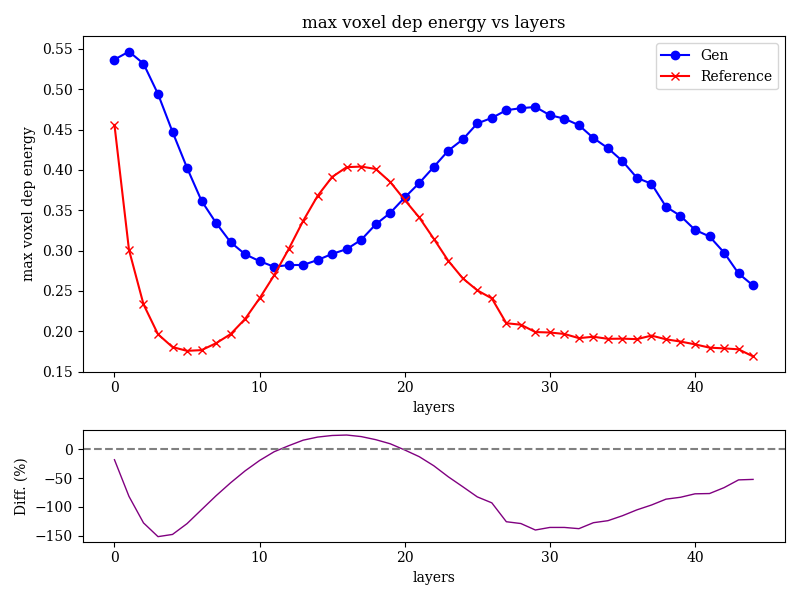
\includegraphics
        [width=\textwidth]{Figures/a1_5.png}
        \caption{Max Voxel Deposit vs Layers}
        \label{fig:exp5}
    \end{subfigure}
    \hfill
    \begin{subfigure}[b]{0.3\textwidth}  % Adjust width to fit 3 figures
        \centering
        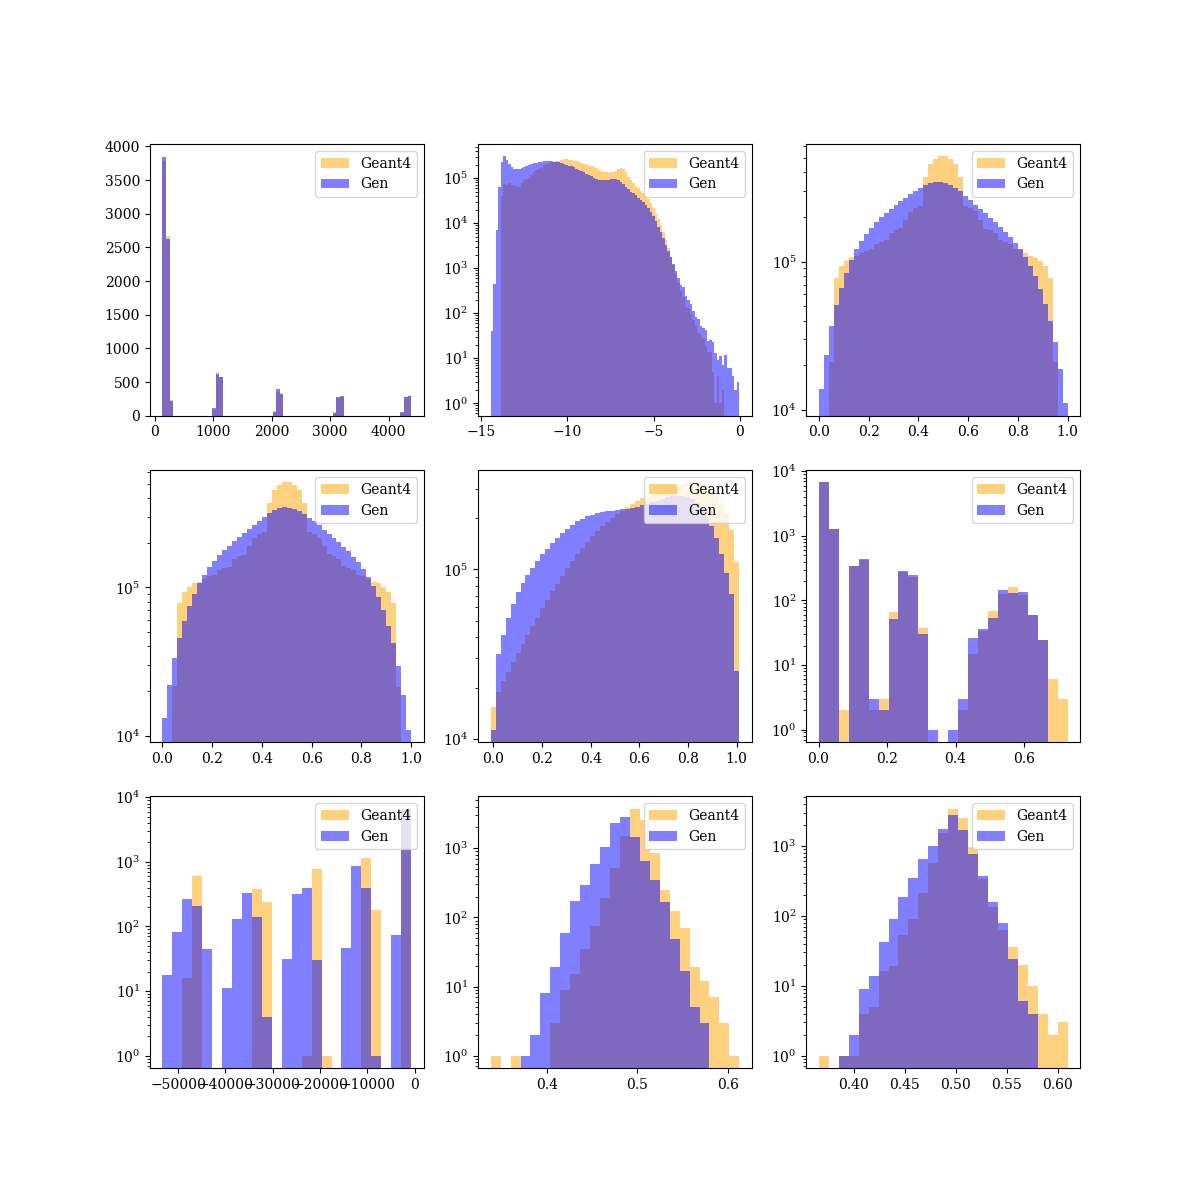
\includegraphics
        [width=\textwidth]{Figures/exponential1.png}
        \caption{1D Histogram}
        \label{fig:exp1}
    \end{subfigure}
    \hfill
    \begin{subfigure}[b]{0.3\textwidth}
        \centering
        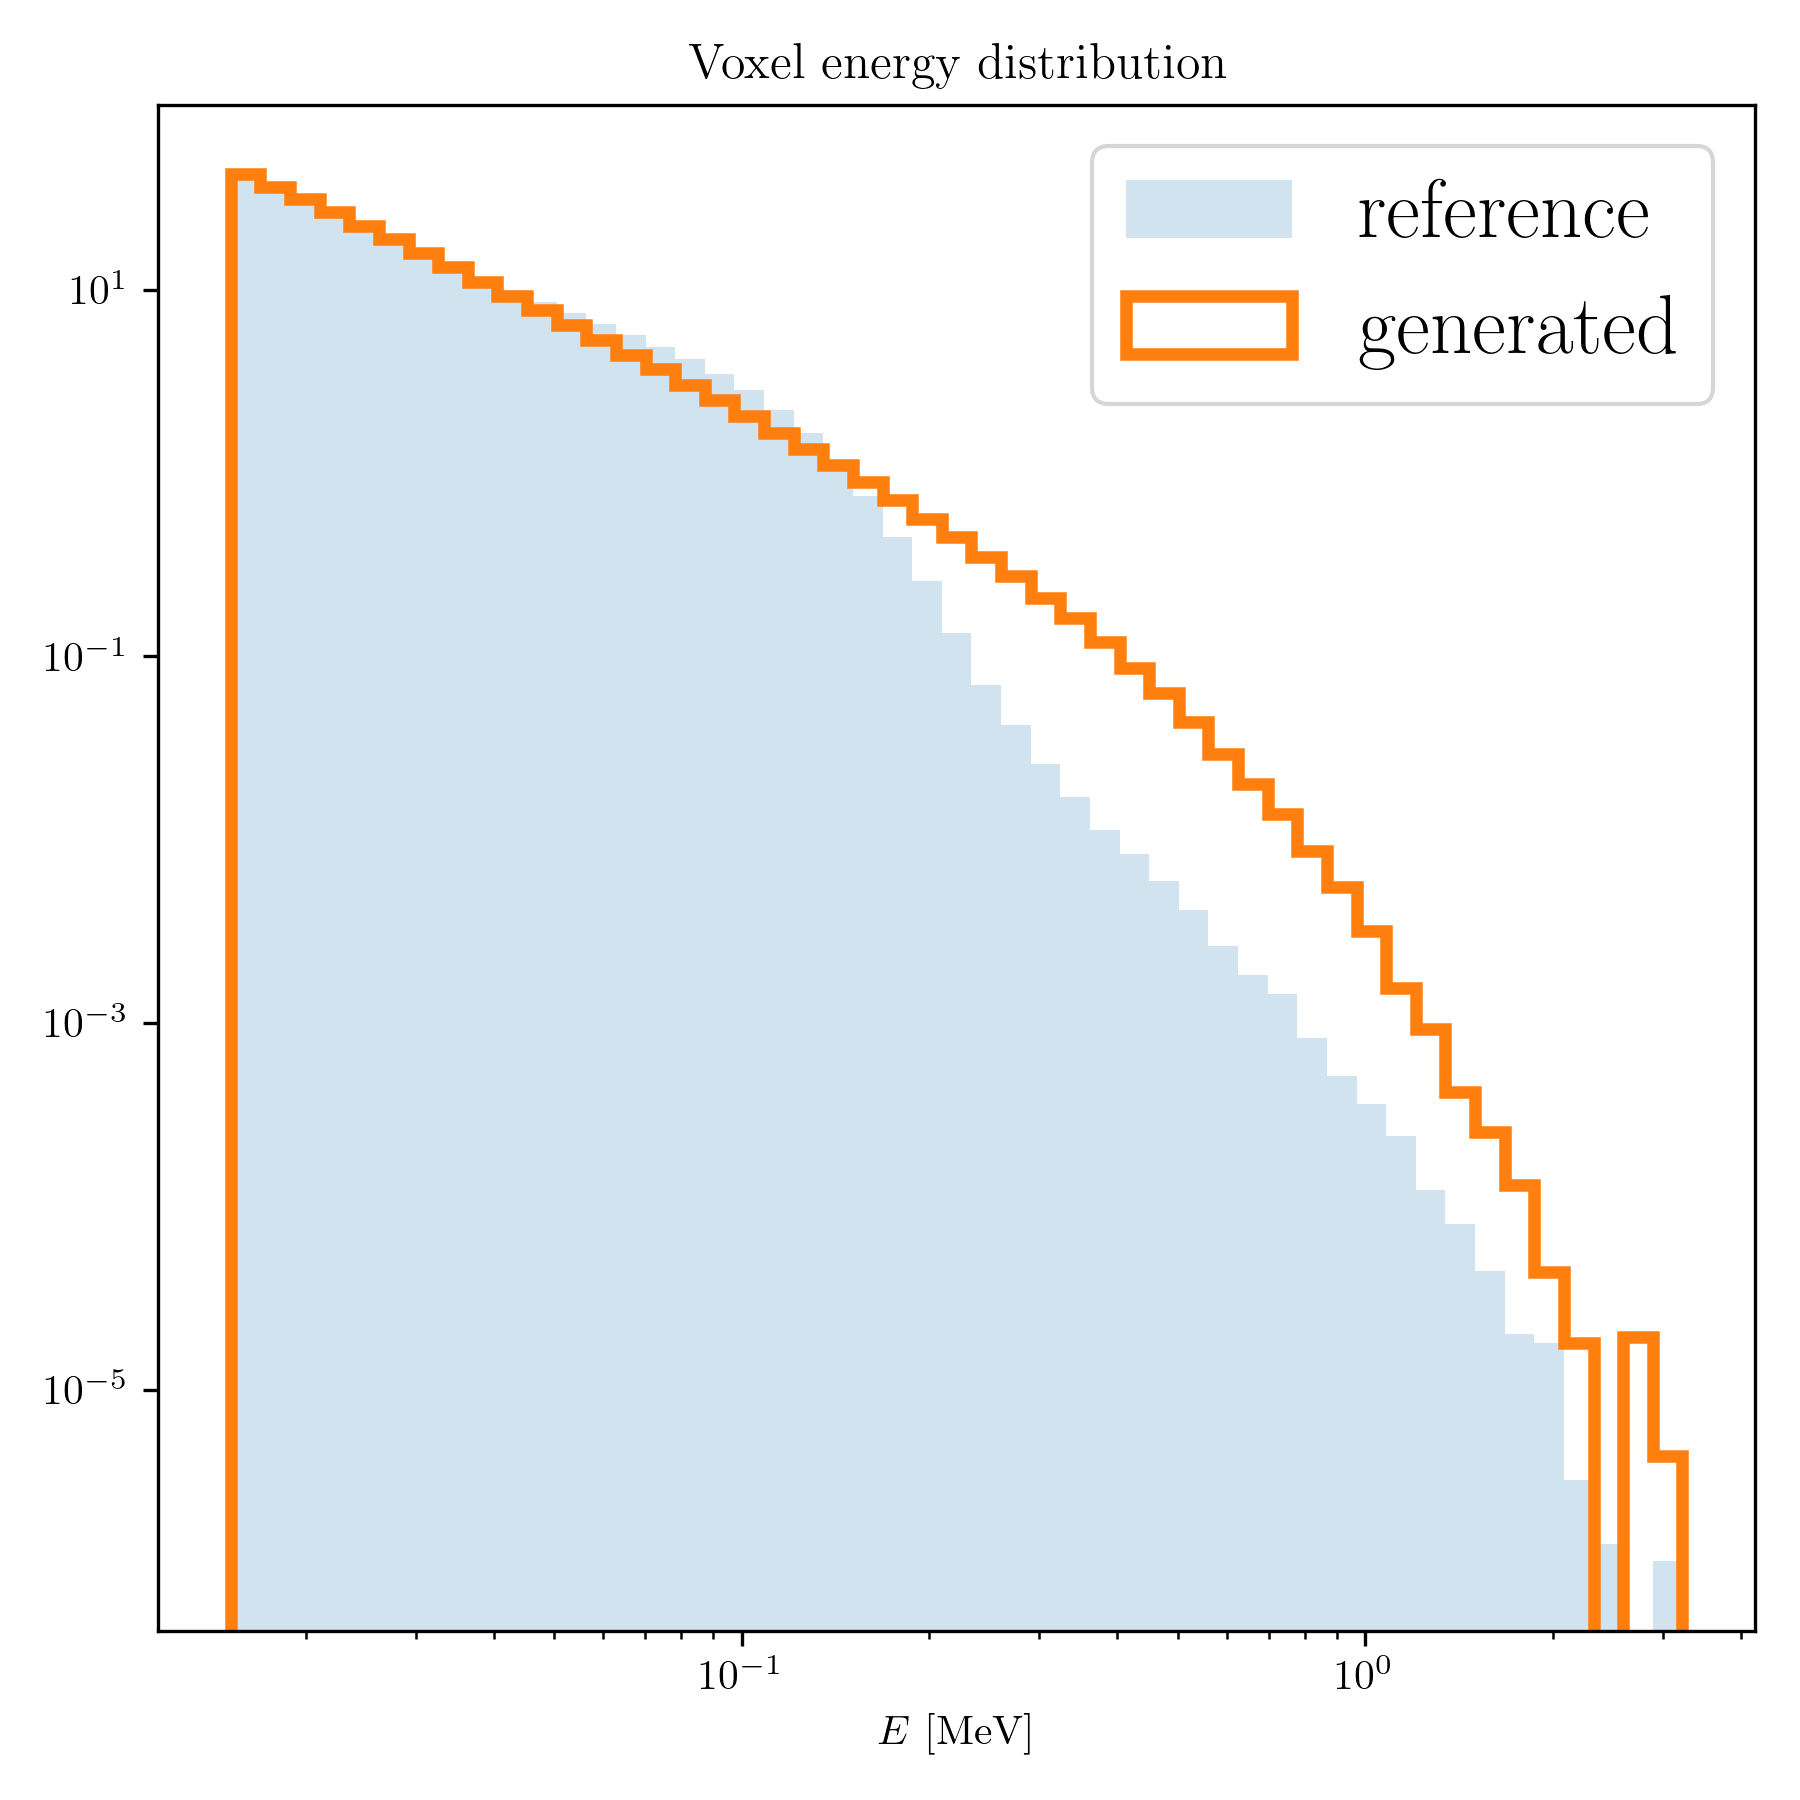
\includegraphics[width=\textwidth]{Figures/exponential6.png}
        \caption{Energy Deposit}
        \label{fig:exp6}
    \end{subfigure}
    \caption{Result for using exponential preprocessor}
\end{figure}

\newpage
\section{Result for using different SDE settings}
every 7 pictures for VE,VP for sde =1,5,10,20. Total 7*2*4=56 pictures
